\documentclass[10pt]{article}
\pdfoutput=1 

\addtolength{\oddsidemargin}{-.875in}
\addtolength{\evensidemargin}{-.875in}
\addtolength{\textwidth}{1.75in}

\addtolength{\topmargin}{-.875in}
\addtolength{\textheight}{1.75in}

\openup 1em

%macro for commenting
\usepackage{color}
\newcommand{\leo}[1]{{\color{blue}{\it leo: #1}}}

\newcommand{\Xbeta}{ X_i^T \beta}
\newcommand{\xbeta}{ x_i^T \beta}


\usepackage[round]{natbib}

\usepackage{rotating}
\usepackage{graphicx}
\usepackage{subcaption}

\usepackage{float}


\usepackage{amsthm,amsmath} 
\usepackage{amssymb}
\usepackage{subcaption}

\newtheorem{theorem}{Theorem}
\newtheorem{lemma}{Lemma}
\newtheorem{corollary}{Corollary}
\newtheorem{remark}{Remark}

\newcommand{\James}[1]{\textcolor{red}{JEJ: #1}}
\DeclareMathOperator{\var}{var}


\usepackage{algorithm}
\usepackage{algpseudocode}


\thispagestyle{empty}
\baselineskip=28pt

\title
{{Calibrated Data Augmentation for Scalable \\ Markov Chain Monte Carlo}}


\author{
     Leo L. Duan,
     James E. Johndrow,
     David B. Dunson
    % \textsuperscript{*}\footnotemark[2]\and
}

 
\begin{document}
    
\maketitle


{\bf Abstract:} Data augmentation is a common technique for building tuning-free Markov chain Monte Carlo algorithms. Although these algorithms are central to applied Bayesian statistics, 
 mixing is often slow in large sample sizes. %leading to poor computational efficiency.  The poor performance can be largely attributable to a mismatch between the rate of convergence of the posterior distribution conditionally on augmented data and with augmented data marginalized out.  
This phenomenon has been attributed to a discrepancy between the rate of posterior contraction and the rate at which typical step sizes converge to zero as the sample size increases. 
In this article, we propose a calibrated data augmentation algorithm, which amplifies the scale of the parameters conditional on the latent data to remove this discrepancy.  Amplification of the scale can introduce bias in the stationary distribution, but we show that suitable tuning parameters can be chosen to bound the approximation error while significantly accelerating mixing.  In addition, bias-free algorithms can be obtained through a Metropolis-Hastings step.  Our approach is applicable to many existing data augmentation algorithms, and we focus on three important examples: probit, logistic and Poisson log-linear. Theoretical support is provided and dramatic gains are shown in applications.
\vskip 12pt

%\baselineskip=12pt
%\par\vfill\noindent
{\noindent  KEY WORDS:  Albert and Chib; Approximate Markov chain Monte Carlo; Big $n$; Data Augmentation; Maximal Correlation; Polya-Gamma; Scaling limits.}
%\par\medskip\noindent
%\clearpage\pagebreak\newpage
\pagenumbering{arabic}

\section{Introduction}
With the deluge of data in modern application areas, there is a pressing need for scalable computational algorithms for inference, including uncertainty quantification.  Somewhat surprisingly, even as the volume of data increases, uncertainty often remains sizable. Examples include financial fraud detection \citep{ngai2011application}, disease mapping \citep{wakefield2007disease} and online click-through tracking \citep{wang2010click}.  Bayesian methods provide a useful paradigm for quantifying uncertainty in these and other large scale applications.

Markov chain Monte Carlo (MCMC) and related sampling algorithms remain the dominant paradigm for Bayesian computation. Although computationally scalable, alternatives such as variational Bayes perform poorly in uncertainty quantification (e.g. Titterington XXX). Conversely, conventional MCMC algorithms offer superior uncertainty quantification but generally scale poorly in the number of parameters $p$ and observations $n$. The computational complexity of MCMC is determined by two factors: the evaluation cost at each sampling iteration and the total number of iterations needed to obtain an acceptably low Monte Carlo error. The former is associated with classical algorithmic complexity, while the latter is a property of the Markov transition kernel. In general, both factors contribute to increasing computational complexity of MCMC as sample size increases, since cost per iteration is rarely independent of $n$, and convergence properties of most MCMC transition kernels tend to degrade with $n$.  %As an analogy to travel in the real world, the former is the speed and the latter is the path distance to reach and tour the target.  Any scaling obstacle in either factor will make MCMC inapplicable. 

A substantial literature focuses on general strategies reducing cost per iteration (\cite{minsker2014robust,srivastava2015wasp,conrad2015accelerating} among others) through accelerating or parallelizing sampling.  %However, very little attention has been paid to the problem of finding an efficient path to reach and explore the target distribution in big data settings. 
%The problem of improving mixing in 
On the other hand, reducing or eliminating the effect of sample size on MCMC convergence is often problem-specific. [Examples?] For example, many routinely used algorithms, such as data augmentation samplers for probit \citep{albert1993bayesian} and logistic models \citep{polson2013bayesian}, can suffer from slow mixing for large sample sizes (see \cite{rajaratnam2015mcmc} and \cite{johndrow2016inefficiency} for details), while alternative Metropolis-Hastings algorithms have mixing properties that are nearly independent of sample size. However, in complex hierarchical models, tuning Metropolis-Hastings proposals is often exceedingly difficult, so there remains no general solution to the large sample MCMC mixing problem for generalized linear models.

%Such issues provide motivation for the development of algorithms for accelerating mixing in large sample size $n$ settings.  
In this article, we focus on improving data augmentation (DA) based MCMC algorithms.  Letting $\pi( \theta | y )$ denote the posterior distribution of the parameters $\theta$ given data $y$, such algorithms focus on the modified stationary distribution $\pi( \theta, z | y ),$ with latent data $z$ introduced in a careful manner so that $\pi( \theta | y) = \int \pi( \theta, z | y ) dz$ and posterior sampling based on the conditional posterior distributions $\pi(z | \theta, y)$ and $\pi( \theta | z, y)$ is easier than directly sampling based on $\pi( \theta | y)$.   For example, after data augmentation a simple blocked Gibbs sampler may be possible, while sampling based on the non-augmented posterior $\pi( \theta |y)$ may require substantial tuning.  DA algorithms are used routinely, with the algorithms of \cite{albert1993bayesian} for probit models and \cite{polson2013bayesian} for logistic regression and Poisson log linear models particularly popular.  

% Such issues provide motivation for the development of algorithms for accelerating mixing in large sample size $n$ settings.  In this article, we focus on improving data augmentation (DA) based MCMC algorithms.  Letting $\pi( \theta | y )$ denote the posterior distribution of the parameters $\theta$ given data $y$, such algorithms focus on the modified stationary distribution $\pi( \theta, z | y ),$ with latent data $z$ introduced in a careful manner so that $\pi( \theta | y) = \int \pi( \theta, z | y ) dz$ and posterior sampling based on the conditional posterior distributions $\pi(z | \theta, y)$ and $\pi( \theta | z, y)$ is easier than directly sampling based on $\pi( \theta | y)$.   For example, after data augmentation a simple blocked Gibbs sampler may be possible, while sampling based on the non-augmented posterior $\pi( \theta |y)$ may require substantial tuning.  DA algorithms are used routinely, with the algorithms of \cite{albert1993bayesian} for probit models and \cite{polson2013bayesian} for logistic regression and Poisson log linear models particularly popular.  

The broad use of such DA algorithms is well justified given their simplicity, lack of tuning and good performance in a broad variety of settings.  However, as the sample size $n$ increases, substantial mixing problems can arise due to a mis-calibration issue.  In particular, it is often the case that as $n$ increases, the conditional posterior $\pi( \theta | z, y)$ concentrates at a faster rate than the marginal posterior $\pi( \theta | y)$. {\color{red} With $\pi(  z|\theta y)$ strongly dependent on the previous state of $\theta$}, this can cause the step size of MCMC algorithms for updating $\theta$  to be much too small.  Special cases of this pitfall of DA are well known in the literature.  For example, the \cite{albert1993bayesian} DA algorithm for probit models for ordered categorical data updates latent threshold parameters from their uniform conditional posterior given the augmented data.   As $n$ increases, these uniform distributions have small support heavily correlated with the previous threshold value, leading to critical mixing problems even in moderate samples.  In this specialized setting, it is common to marginalize out $z$ in updating the latent thresholds using a Metropolis-Hastings (MH) step \citep{cowles1996accelerating}. In this article, our focus is on obtaining a broad and more fundamental solution to the mis-calibration problem.

There is a previous literature attempting to accelerate mixing in DA algorithms through the use of parameter expansion (PX) \citep{liu1999parameter}.  The basic idea of PX-DA is that poor mixing is often due to high posterior dependence in parameters, which are updated separately within an MCMC algorithm.  By introducing extra or redundant parameters into the MCMC algorithm, it is possible to dilute correlations in the parameters of interest and obtain improved mixing.  PX-DA versions of the popular \cite{albert1993bayesian} algorithm have been developed \citep{liu1999parameter}, leading to some gains.  

However, PX-DA does not address the mis-calibration issue, which is the focus of this article.  In particular, we propose a calibrated DA (CDA) class of algorithms, which {\color{red} removes the dependency of the latent variable on the parameter, or} calibrates the transition variance in the posterior $\pi( \theta | z, y)$ by adjusting the conditional variance.  These adjustments can very significantly reduce autocorrelation in the Markov chain, dramatically improving mixing relative to DA or PX-DA in many very large $n$ settings. Calibrating the variance leads to a bias in the stationary distribution so that the target is $\pi_r( \theta | y)$, which may differ slightly from $\pi( \theta | y)$.  Metropolis-Hastings adjustment is employed to eliminate bias. We also show in several cases, this approximation error can be analytically bounded with suitable choice of the working parameter, leading to fast-mixing approximate MCMC. The proposed CDA approach is widely applicable, and we demonstrate the utility through probit, logistic and Poisson log-linear examples.


Section 2 proposes the general calibrated data augmentation (CDA) algorithm. Section 3 presents theory showing acceleration of mixing, accuracy of approximation, and ergodicity for the approximate MCMC algorithm without use of a MH adjustment.  Section 4 provides simulation experiments and comparisons with existing algorithms.  Section 5 contains an application to a large computational advertising data set. All the proofs are provided in the appendix. %check again

\section{Calibrated Data Augmentation}

The primary role of data augmentation (DA) in MCMC algorithms is to make Gibbs sampling possible, because after augmentation conditional posterior distributions follow parametric forms that are easy to sample from.  DA Gibbs proceeds by sampling from the conditional posterior distributions of the latent data based on $\pi(z| \theta,y)$ and from conditional posterior distributions of the parameters based on $\pi(\theta | z,y)$; each of these sampling steps can be broken up into a series of conditional updates for successive subsets of the latent data and parameters when the joint conditionals $\pi(z|\theta,y)$ and $\pi(\theta | z, y)$ are not available in a simple form.

The current article focuses on problems that arise due to a mis-calibration problem that occurs when {(i) \color{red} $z$ is strongly dependent on the last value of $\theta$, and (ii) $\var(\theta | z,y)$ is substantially less than $\var( \theta | y)$.  The first condition is very common in Gibbs sampling due to the use of full conditional distributions.} The second condition is related to the rate difference of the concentration.  Consider that the conditional posterior given the latent data is obtained by updating the posterior given the observed data with information in the latent data likelihood via Bayes rule as: $\pi( \theta | z, y) \propto \pi( \theta | y) L( z | \theta, y)$.  Hence, as the amount of information in the latent data likelihood $L(z | \theta, y)$ increases, which typically occurs as the observed data sample size $n$ increases, $\var(\theta | z,y) \ll \var( \theta | y)$.  The combination of these two conditions naturally leads to a slow mixing problem, because the MCMC updates based on $\pi(\theta | z,y)$ will only explore a small region of $\pi( \theta | y)$.  In general, the problem gets worse as the information in the latent data likelihood increases; inefficiency can arise even in moderate sample sizes but becomes critical in large samples. \James{there is a sizable literature on ``fraction of missing information'', which I think is related and we need to cite}

The key novel idea of this article is to {\em calibrate} DA by adjusting the step size of the conditional distribution. Addressing either one of the conditions mentioned above leads to substantial acceleration. To remove the dependency of the latent variable on the last state,  the calibrated DA (CDA) first marginalizes out the parameter from the Markov chain and then samples the parameter as an extra step at the end of each iteration. To calibrate the rate mismatch in the conditional posterior covariance, CDA induces an increase in $\var( \theta | z,y)$ by  inflating the variance parameter with a working parameter $r$. This leads up to an altered likelihood $\pi_r(y|\theta)= \int \pi_r(y|\theta,z)\pi_r(z)dz$. To reduce the bias, a correction term $b$ is introduced so that $\pi_{r,b}(y|\theta)$ is close to $\pi(y|\theta)$. The samples from $\pi_{r,b}(y|\theta)$ can be used as either as approximate posterior or good proposal in the Metropolis-Hastings algorithm. We demonstrate a general numeric algorithm for $\pi(\theta | y,z)$ in the location-scale family, as well as analytical method for some special cases.

We now illustrate the two calibration strategies. As the parameters are commonly in multiple dimensions, we now divide the parameter into two sets $\theta=\{\theta_1,\theta_2 \}$. Let $\theta_1$ be the ones that mixes slowly.



\subsection{Removing Dependency by Marginalization}

Intuitively, if $\theta_1$ concentrates rapidly near a function of $z$, but $z$ depends on the last value of $\theta_1$, slow mixing naturally occurs. Breaking the dependency would lead to significant improvement. The first strategy involves marginalize out $\theta_1$ in the conditional distribution of  $z$ and $\theta_2$, then  sample new $\theta_1$ based on $\pi(\theta_1|z,\theta_2,y)$, shown in Algorithm~\ref{integration_cda}:

\begin{algorithm}[H]
\caption{Marginalization based CDA}
\label{integration_cda}
\begin{algorithmic}
\State Based on the augmented joint distribution $\pi (z,y,\theta_1,\theta_2)$, obtain the marginal $\pi (z,y,\theta_2)=\int\pi (z,y,\theta_1,\theta_2) d\theta_1$.
\State \For{ $step=1\ldots N_{Steps}$ }
\State Sample $z$ from the marginal $\pi(z|\theta_2, y)$;
\State Sample $\theta_2$ from the marginal $\pi(\theta_2|z, y)$;
\State Sample $\theta_1$ from the full conditional $\pi(\theta_1|z,\theta_2, y)$;
\EndFor
\end{algorithmic}
\end{algorithm}

Obviously, this does not change the stationary distribution, but the sampling of the latent variable $z$ no longer relies on the previous value of $\theta_1$. Therefore the generation of the new $\theta_1$ is free from its last state.

This integration strategy is similar to the collapsed sampler proposed by \cite{liu1994collapsed},  who focused on accelerating the imputation of $z$ as the missing data by marginalizing out the the unimportant variables. The key difference is that $\theta_1$ is important but marginalized out at first to exclude the information of the past, then it is sampled again at the end of each MCMC iteration. Note the first two steps in the algorithm  already form a complete Markov chain and neither $\pi(z|\theta_2, y)$ or $\pi(\theta_2|z, y)$ depends $\theta_1$. Therefore the autocorrelation of $E(\theta_1|z,\theta)$ is significantly reduced. A more rigorous theory will be provided in the next section.

\begin{remark}
Due to the closed-form of $\pi(\theta_1| \theta_2,z,y)$ is commonly available in Gibbs sampling, it is possible to marginalize $\theta_1$ out in most cases. The easiness of applying the new algorithm depends on if the marginal $\pi(z|\theta_2, y)$ and $\pi(\theta_2|z, y)$ can be readily sampled. When this is not true, it is possible to make some compromises such as reverting $\theta_2$ to $\pi(\theta_2|\theta_1,z, y)$, as long as $\theta_2$ does not impact greatly on the concentration of $\theta_1$.
\end{remark}

We use the next example to show if $\pi(\theta_1| \theta_2,z,y)$  follows uniform distribution, the marginalization does not alter the distribution forms of the other posteriors, but leads to significant gains in mixing. Therefore, under such cases marginalization is always recommended.

{\bf Example 1: Threshold Updating in Ordinal Probit Regression}

Consider the \cite{albert1993bayesian} DA algorithm for the probit regression with ordered categorical data, as aforementioned in the introduction. The likelihood is $L(y_i=j|x_i,\beta,\gamma)= \{  \Phi( \gamma_j- x^T_i\beta) -  \Phi( \gamma_{j-1}- x^T_i\beta)    \}$, where $\Phi$ is the cumulative distribution function of standard normal, $\gamma=\{\gamma_0,\gamma_1,...\gamma_k\}$ are the threshold parameters that correspond to the boundaries of $k$ categories, with $\gamma_0=-\infty$, $\gamma_k=-\infty$. To ensure identifiability, $\gamma_1$ is fixed at $0$. A latent variable was discovered as the truncated normal distribution conditioned on $\beta$ and $\gamma$, $z_i \sim \mathcal N_{(\gamma_{j-1}, \gamma_{j})}(x^T_i\beta,1)$. For simplicity, flat priors are assumed for both $\beta$ and $\gamma$. Thanks to the augmentation, the posterior for the other parameters  can be sampled from  normal $\beta \sim \mathcal{N} \{   (x^Tx)^{-1}(x^Tz),(x^Tx)^{-1} \}$ and uniform $\gamma_j \sim \mathcal{U}\{ \underset{i:y_i=j}{\max}(z_i),  \underset{i:y_i=j+1}{\min} (z_i)  \}$.

In the conditional distribution $\pi( z|\gamma,\beta,y) $, both the maximum of $z_i \sim \mathcal N_{(\gamma_{j-1}, \gamma_{j})}(x^T_i\beta,1)$ and the minimum of $z_i \sim \mathcal \mathcal{N}_{(\gamma_{j}, \gamma_{j+1})}(x^T_i\beta,1)$ approach rapidly to the boundary $\gamma_j$ as the numbers of $y_i=j$ and $y_i=j+1$ increase. Immediately at the next step,  $\pi( \gamma_j| z,y) $ is confined by those two values. This causes critical mixing issue. To illustrate, we simulate only $1,000$ data points with $x_i^T\beta \sim \mathcal{N}(-1,1)$ and threshold $\{-\infty, 0, 1, \infty\}$, obtaining 3 categories with count $504$, $267$ and $229$. Even on this small sample with relatively balanced data, the estimated threshold $\gamma_2$ is critically slow (Figure~\ref{ordered_probit}).

Following Algorithm~\ref{integration_cda} with $\theta_1=\{ \gamma_2,\ldots \gamma_{k-1}\}$ and $\theta_2=\beta$, CDA first integrates the joint distribution $\pi(z,y,x,\beta,\gamma,y)= \prod_i  {\mathcal N} (z_i |x^T_i\beta,1)   \prod_{j=1} \frac{1 \{ \underset{i:y_i=j}{\max}(z_i) < \gamma_j< \underset{i:y_i=j+1}{\min} (z_i) \}}{\underset{i:y_i=j+1}{\min} (z_i) -\underset{i:y_i=j}{\max}(z_i) }$ over $\gamma_2,\ldots \gamma_{k-1}$, where each uniform simply integrates to $1$. The resulting algorithm is 

\begin{equation}
	\begin{aligned}
	&	z_i \sim  {\mathcal N}_{(-\infty,0)} (x^T_i\beta,1) \text{ if $y_i=1$},\\
	&	z_i \sim {\mathcal N}_{(0,\infty)} (x^T_i\beta,1) \text{ if $y_i>1$},\\
	&	\beta \sim \mathcal{N} \{   (x^Tx)^{-1}(x^Tz),(x^Tx)^{-1}  \} ,\\
	& \gamma_j\sim U(  z_{\big(\sum_i 1(y_i \le j) \big)}, z_{\big(\sum_i 1(y_i \le j)+1 \big)}), 
	\end{aligned}
\end{equation}
where $z_{\big(m\big)}$ denotes the $m$th order statistics. Due to the removal of correlation from the past, the mixing is substantially improved (Figure~\ref{ordered_probit}).



\begin{figure}[H]
 % \centering
  \begin{subfigure}[b]{0.49\textwidth}
 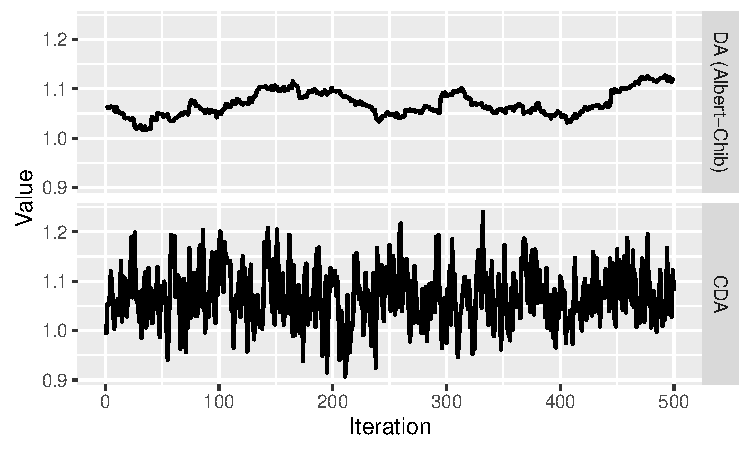
\includegraphics[width=1\textwidth]{ordered_probit_trace_plot.pdf}
  \caption{Traceplot illustrating mixing performance of the original DA and CDA algorithms in the threshold updating in probit regression with ordered categorical data.}
\end{subfigure}
  \hfill
   \begin{subfigure}[b]{0.49\textwidth}
 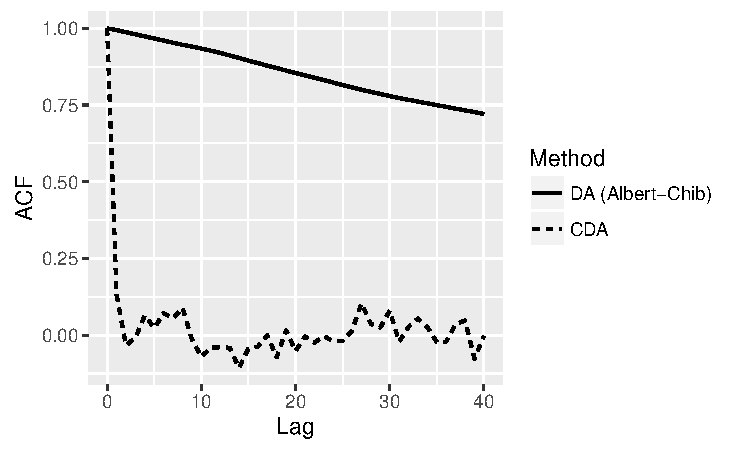
\includegraphics[width=1\textwidth]{ordered_probit_acf.pdf}
  \caption{Autocorrelation function (ACF) illustrating that the calibration improves the mixing from high correlation in $40$ lags to an immediate drop to low correlation.  
  }¡
\end{subfigure}
 \caption{Panel (a) demonstrates the improvement in mixing and panel (b) shows autocorrelations change by calibrating  \cite{albert1993bayesian} algorithm with threshold updating in ordered categorical data.}
  \label{ordered_probit}
 \end{figure}
 

\subsection{Fixing Variance Mismatch by Adjusting Conditional Variance}

CDA can directly correct the mismatch between the marginal and conditional variances. This relies on increasing the conditional variance via an approximate distribution. We assume the adjusting does not impact the posterior of $\pi(\theta_2|\theta_1,z,y)$ and hence omit it in this section for simplicity. CDA first induces an increase in $var(\theta|z,y)$ by modifying the parameters in each $\pi(z_i|\theta)$ with an working parameter $r_i$. For example,  when $var(\theta|z,y)$ is a linear function of the $var(z_i|\theta)$ (e.g. $var(\theta|z,y)= [ x^{T} diag \{ 1/ var(z_i|\theta)\}x ]^{-1}$), it is replaced with the $r_i  var(z_i|\theta)$; when $var(\theta|z,y)$ is related to $z_i$  (e.g.  $var(\theta|z,y)= [ x^{T} diag \{z\}x ]^{-1}$), we change the parameters in $\pi(z_i|\theta)$ to generate smaller $z_i$. Let subscript $r$ denote the modified ones. The modified marginal likelihood is obtained for each $L_r(y_i|\theta)= \int \pi(y_i, z_i | \theta) d z_i$. Without loss of generality, we assume that variance is monotonically increase in $r>1$ and $r=1$ corresponds to no change. 

With the same distributional form, the integration will have the same distribution as $L(y_i|\theta)$ with difference parameters. Comparing the two, a bias correction term $b_i$ is used to quantify the difference. For example, if $L(y_i|\theta)$ and $L_r(y_i|\theta)$ differs in the parameter as $x_i^T\theta$ and  $\sqrt{r_i} x_i^T\theta$, then the second term is replaced as $\sqrt{r_i} x_i^T\theta+ b_i$ with  ideal bias correction  near $(1-\sqrt{r_i}) x_i^T\theta$. Then new the correction parameter is passed down in deriving the posterior $\pi_{r,b}( z_i | y_i, \theta )$ and $\pi_{r,b}( \theta |z,y)$.

With fixed $r$ and $b$, the posterior sample from the new $\pi_{r,b}(\theta|y)$ is an approximate to the $\pi(\theta|y)$. To reduce the approximation error, the numeric adaptation can be made on $r_i$ and $b_i$ to increase $L_{r,b}(y_i\theta)/L(y_i|\theta)$. To obtain exact posterior, the sample from $\pi_{r,b}(\theta|y)$ can be used as proposal in Metropolis-Hastings step. Due to the similarity of the proposal to the true density, the proposed new parameter can be in multiple dimensions while enjoys high acceptance rate. In some special cases, analytical solution exists for good values of $r_i$ and $b_i$ with negligible approximation error, then the sample of $\pi_{r,b}(\theta|y)$ can be as the approximate posterior sample without the accept-reject step.

\subsubsection{Numeric Method}

We first present a general method that works in most of the DA algorithms that requires calibration. This involves numeric adaptation of the working parameters $r$ and $b$. The algorithm is listed in Algorithm~\ref{numerical_cda}. After the variance and bias adjustment terms are included, the procedures consists of two parts: in the tuning period, $r$ and $b$ are adapted using $L_{r,b}(y_i\theta)/L(y_i|\theta)$ at each step; in the sampling period, those parameters are fixed to ensure ergodicity.
 
 
\begin{algorithm}[H]
		\caption{Variance Adjusting CDA (Numeric)}
		\label{numerical_cda}
		    \begin{algorithmic}
		\State Increase the variance of $\pi(\theta| z,y)$ by changing the parameter in $\pi(z_i |\theta,y_i)$ with $r_i$;
		\State Integrate the modified density to obtain $L_r(y_i|\theta)= \int \pi_r (z_i|\theta) \pi(y_i|z_i,\theta) d z_i$; 
		\State Compare with $L(y_i|\theta)$, include another bias correction parameter $b$ so that $L_{r,b}(y_i|\theta)$ can be equal to $L(y_i|\theta)$ with some $b$ for all $r$.
		\State Derive the analytical form of $f_b(\theta,y_i,r_i)$ so that $L_{r,b={f_b(\theta,y_i,r_i)}}(y_i|\theta)=L(y_i|\theta)$;
		\State Obtain $\pi_{r,b}(z_i|\theta, y_i)$ and  $\pi_{r,b}(\theta| z, y)$;
		\State Initialize $r_i$ to a large value and $b_i= f_b(\theta,y_i, r_i)$  for $i=1\ldots n$;
		\State \For{ $step=1\ldots N_{Steps}$ }
		\State Generate individual $z_i$ from $\pi_{r,b}(z_i|\theta, y_i)$;
		\State Generate $\theta'$ from $\pi_{r,b}(\theta'|z, y)$;
		\State Compute $\alpha_i = \frac{L( y_i|\theta', z_i ) }{L( y_i|\theta, z_i )}$  for $i=1\ldots n$;
		\State Set $\theta=\theta'$ if $\mathcal{U}(0,1)< \frac{Q(\theta',\theta)}{Q(\theta,\theta')}\prod \alpha_i$, where $Q(\theta,\theta') = \int  \pi_{r,b}(\theta| z, y) \pi_{r,b}(z|\theta', y)d z$
		\State \If{$step<N_{Tuning}$}
			\State Set $b_i= f_b(\theta,y_i, r_i)$ for $i=1\ldots n$;
			\State If $\alpha_i<1$, set $r_i$ to $1 \vee (r_i \alpha_i)$  for $i=1\ldots n$;
		\EndIf
		\EndFor
		\end{algorithmic}
\end{algorithm}

\begin{remark}
The algorithm is generally applicable. For example, in the cases where $\pi(z_i | \theta,y_i)$ is in location-scale family, the variance adjustment can be made on the scale parameter while bias correction is applied on the location parameter. In most cases, $\frac{Q(\theta',\theta)}{Q(\theta,\theta')}=1$ due to the symmetry.
\end{remark}

We now use the probit regression to illustrate the numeric method. Due to the conditional $\pi(z_i | \theta,y_i)$ is normal, CDA increases its variance and applies bias correction on the mean.

 {\bf Example 2: Probit Regression with Rare Event}

 
Consider a probit regression $\prod_{i=1}^{n}L(y_i|\xbeta)= \prod_{i=1}^n \Phi(\xbeta)^{y_i} \{ 1-\Phi(\xbeta) \} ^{(1-y_i)}$ with rare event so that the total occurrence of $y_i=1$ is quite small compared to to $n$. We use $\beta={-5,1}$ corresponding to the intercept and $x_{i,1}\sim \mathcal{N}(0,1)$ to generate only $29$ positive outcomes among $n=10,000$. The posterior samples from $\beta \sim \mathcal{N} \{   (x^Tx)^{-1}(x^Tz),(x^Tx)^{-1} \}$, conditional on $z_i \sim N_{(-\infty,0)}(\xbeta,1)$ if $y_i=0$ and $z_i \sim N_{(0,\infty)}(\xbeta,1)$ if $y_i=1$. For the intercept term, it concentrates at the rate of $O(1/n)$; while marginally, it concentrates much slower at $O(1/\log n)$. The slow mixing becomes particularly problematic when $n$ is very large, which is common in rare event applications. In this testing case, the \cite{albert1993bayesian} DA algorithm suffers from extremely slow mixing. To compare, we test the parameter expansion algorithm (PX-DA) proposed by \cite{liu1999parameter}, where a redundant parameter is used in the probit link $\Phi(\alpha\xbeta)$. PX-DA reduces the correlation to some extent, however, it does not solve the variance mismatch problem. As shown in Figure~\ref{probit_demo} (a) and (b), both DA and PX-DA result in extremely slow mixing.

Noting $var(z_i| \beta)=1$, CDA algorithm first replaces the it with $r_i > 1$ so that the conditional variance for $\beta$ becomes $(x^T diag^{-1}\{r_i\} x)^{-1}$. The marginalization and adding bias correction leads to $L_{r,b}(y_i|\beta)= \Phi\{  (\xbeta+ b_i)/\sqrt{r_i}  \}^{y_i} [ 1-\Phi\{  (\xbeta+ b_i)/\sqrt{r_i}  \} ] ^{(1-y_i)}$. The resulting algorithm for the proposal is:
 
\begin{equation}\begin{aligned}
&	  z_i \sim N_{(-\infty,0)}(\xbeta+b_i,r_i) \text{ if $y_i=0$ } \\
&	  z_i \sim N_{(0,\infty)}(\xbeta+b_i,r_i) \text{ if $y_i=1$}\\
&    \beta \sim \mathcal{N} \{   (x^T diag^{-1}\{r_i\}x)^{-1},  x^T diag^{-1}\{r_i\}(z-b_i),(x^T  diag^{-1}\{r_i\} x)^{-1} \} 
\end{aligned}\end{equation}

 The calibrated algorithm leads to significant improvement of the mixing (Figure~\ref{probit_demo}a and b). In the numerically adapted proposal distribution (that is close to the true posterior distribution), it is interesting to note the tuned $r_i$ is related to the posterior value of $\xbeta$ (Figure~\ref{probit_demo}c). The very negative $\xbeta$ ($< -4$) suffers the mis-match in the conditional and marginal variance, hence allows large $r_i$ to adjust the step size. The bias correction is linear in $(\sqrt{r_i}-1 ) \xbeta$ as expected (Figure~\ref{probit_demo}d).
 
 
\begin{figure}[H]
 % \centering
  \begin{subfigure}[b]{0.49\textwidth}
 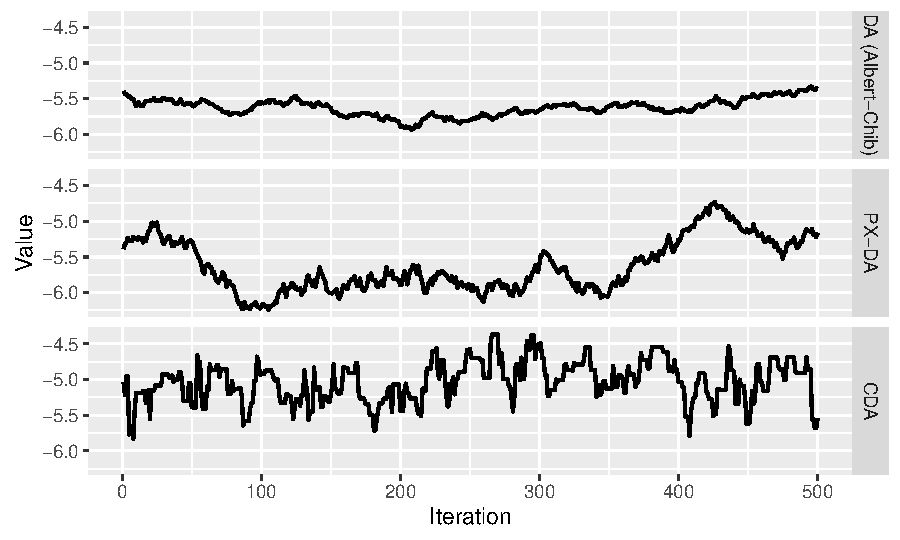
\includegraphics[width=1\textwidth]{probit15_trace_plot.pdf}
  \caption{Traceplot illustrating mixing performance of the original DA, parameter expanded DA and CDA algorithms in probit regression with rare event data.}
\end{subfigure}
  \hfill
   \begin{subfigure}[b]{0.49\textwidth}
 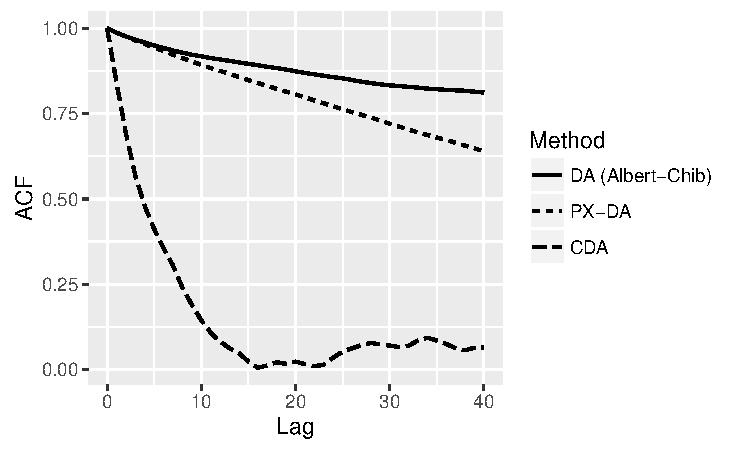
\includegraphics[width=1\textwidth]{probit15_acf.pdf}
  \caption{Autocorrelation function (ACF) illustrating the slow mixing of the DA and parameter expanded DA in rare event data, and CDA correcting this problem.}
\end{subfigure}
   \begin{subfigure}[b]{0.49\textwidth}
 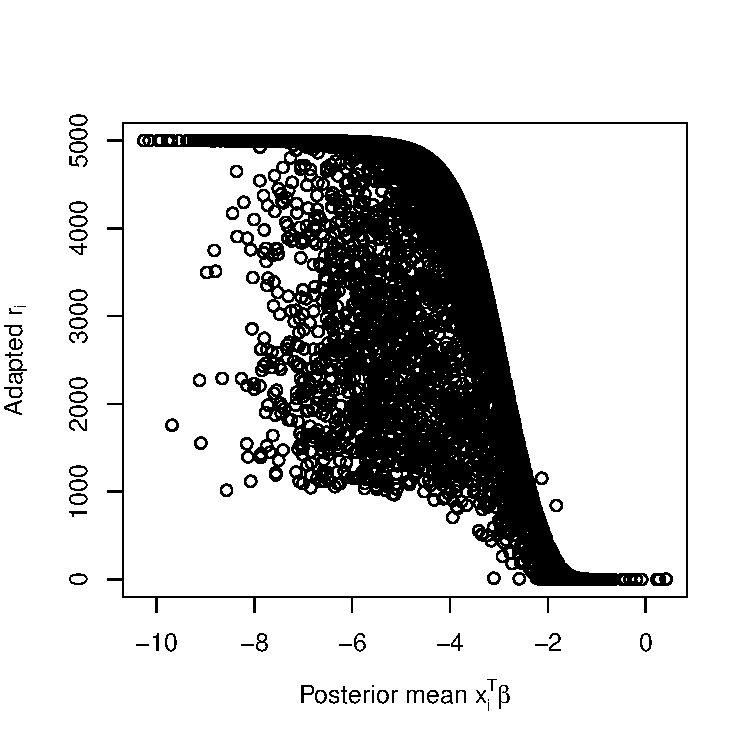
\includegraphics[width=1\textwidth]{probit_cda_r}
  \caption{Numerically optimized $r_i$ showing the room for variance increase is related to the  value of $\xbeta$.}
\end{subfigure}
  \begin{subfigure}[b]{0.49\textwidth}
 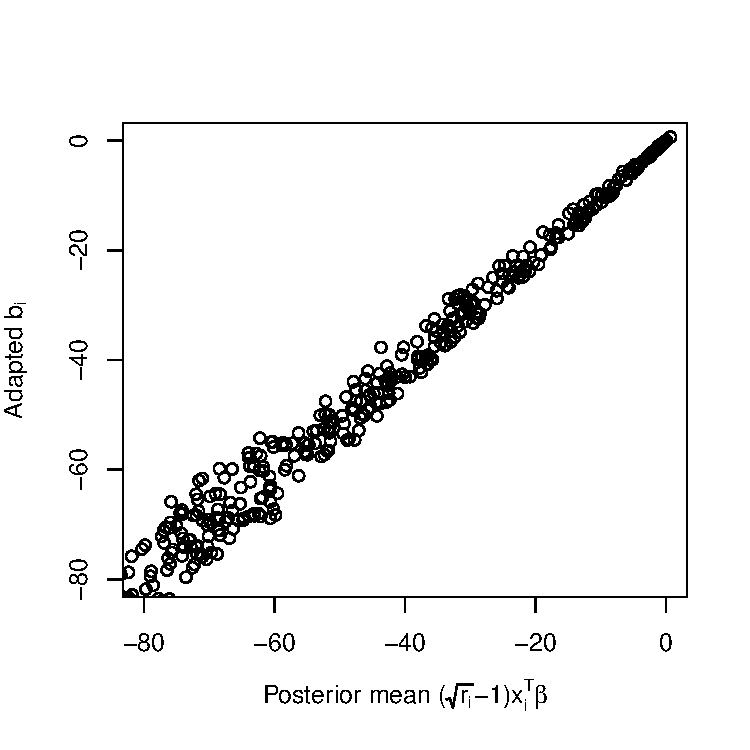
\includegraphics[width=1\textwidth]{probit_cda_b}
  \caption{Numerically optimized $b_i$ in the proposal appearing linear and close to the true bias in $(1-\sqrt{r_i} ) \xbeta$.}
\end{subfigure}
\label{probit_demo}
 \caption{Panel (a) demonstrates in traceplot and panel (b) in autocorrelation about the substantial improvement in CDA by correcting the variance mis-match in probit regression with rare event data, compared with the original \citep{albert1993bayesian} and parameter-expanded methods \citep{liu1999parameter}. Panel (c) shows the degree of the variance increase in $r_i$ (if $r_i=1$: no increase) with respect to the value of $\xbeta$. Panel (d) shows the bias correction term is close to the true bias if no correction were made. }
 \end{figure}
 
\subsubsection{Analytical Approximate Method}

The numeric solution presented above is generally applicable. In some cases, the algorithm can be further simplified to direct sampling without the Metropolis-Hastings step. If the the approximation error can be analytically controlled under a small difference, the approximation ones can be used.

Let $d(\theta, \theta_{r,b})$ be the distance between the two posteriors based on the exact and approximate method. For example, it can be the Kullback-Leibler distance $E\sum_i \{ \log L_{r,b}(y_i | \theta) - \log L(y_i| \theta)\}$. A more loose but useful bound is the norm distance between the first two moments $||\mbox{E}(\theta|y)-\mbox{E}_{r,b}(\theta|y)||$,  $||\mbox{var}(\theta|y)-\mbox{var}_{r,b}(\theta|y)||$. Both criteria would be carefully examined in the next section.

Whether there is an applicable analytical CDA depends on if the bias can be analytically approximated without using $\theta$, at least in a subspace of $\theta$. We found this is the case in several popular distributions, such as logistic, Poisson log-linear and complementary log-log models. The distance is bounded over the posterior sample $\varTheta^*$ for $ \sup_{\theta \in \varTheta^*} d(\theta, \theta_{r,b})\le \epsilon$, using adaptive $r_i$ and $b_i$.


\begin{algorithm}[H]
		\caption{Variance Adjusting CDA (Analytical)}
		\label{numerical_cda}
		    \begin{algorithmic}
			\State Increase the variance of $\pi(\theta| z,y)$ by changing the parameter in $\pi(z_i |\theta,y_i)$ with $r_i$;
		\State Integrate the modified density to obtain $L_r(y_i|\theta)= \int \pi_r (z_i|\theta) \pi(y_i|z_i,\theta) d z_i$; 
		\State Compare with $L(y_i|\theta)$, include another bias correction parameter $b$ so that $L_{r,b}(y_i|\theta)$ can be equal to $L(y_i|\theta)$ with some $b$ for all $r$.
		\State Derive the analytical form of $f_b(\theta,y_i,r_i)$ so that $L_{r,b={f_b(\theta,y_i,r_i)}}(y_i|\theta)=L(y_i|\theta)$;
		\State Check if $f_b(\theta,y_i,r_i)$ can be approximated by $b_i(y_i,r_i)$ in some region of $\theta$.
		\State Initialize $r_i$ to a large value and $b_i$  for $i=1\ldots n$;
		\State \For{ $step=1\ldots N_{Steps}$ }
		\State Generate individual $z_i$ from $\pi_{r,b}(z_i|\theta, y_i)$;
		\State Generate $\theta$ from $\pi_{r,b}(\theta|z, y)$;
		\State If  $ \sup_{\theta \in \varTheta^*} d(\theta, \theta_{r,b})\le \epsilon$ is not satisfied, update $r_i$ and $b_i$;
		\EndFor
		\end{algorithmic}
\end{algorithm}


{\bf Calibration Example 3: Mixed Effects Logistic Regression}

To demonstrate the analytical method, we use the logistic link as an example. Consider a mixed effects logistic regression with  $L(y_i|\beta, \sigma^2)\propto \frac{\exp\{ (\xbeta+s_i^T\gamma_i) y_i \} }{1+ \exp(\xbeta+s_i^T\gamma_i)}$, where $\xbeta$ is the fixed effect with $\beta$ as the parameter of interest, $s_i^T\gamma_i$ is the random effect with $\gamma_{i,j} \stackrel{iid}{\sim} N(0, \sigma_j^2)$ for all $i=1\ldots n$. We use prior $\pi(\beta)\propto 1$ and $\pi(\sigma_j)=\sigma_j^{-2}$. The Polya-Gamma DA proposed by \cite{polson2013bayesian} samples from $z_i\sim \mathcal{PG}(1, \xbeta+s_i^T\gamma_i)$, $\gamma_i \sim \mathcal{N}\{  (s_i z_i s_i^T   + diag\{\sigma_j^{-2}\}  )^{-1}   s_i  (y_i-\frac{1}{2} - z_i \xbeta)  ,  (s_i z_i s_i^T   + diag\{\sigma_j^{-2}\}  )^{-1}   \}$, $\sigma_j^{2}\sim \mathcal{IG}(n/2, \sum_i \gamma_{ij}^2/2)$ and lastly $\beta \sim N\{  (x^T diag\{z_i\}x)^{-1}   x^T  (y-\frac{1}{2} -  z_i vec \{ s_i^T\gamma_i \})  ,  (x^T diag\{z_i\}x)^{-1}   \}$. Like the probit regression, slow mixing emerges when $\sum y_i$ is small compared to $n$.

CDA adjusts the conditional variance $(x^T diag\{z_i\}x)^{-1} $ by reducing the the value of $z_i$. To achieve this, the original Polya-Gamma distribution is replaced by  $z_i\sim \mathcal{PG}(\frac{1}{r_i}, \xbeta+s_i^T\gamma_i + b_i)$ with $r_i>1$ and $b_i$ as the bias-correction term. The integration leads to $L_{r,b}(y_i|\beta, \sigma^2)\propto \frac{\exp\{ (\xbeta+s_i^T\gamma_i) y_i \} }{ \{ 1+ \exp(\xbeta+s_i^T\gamma_i +b_i) \}^{1/r_i} }$. Setting $L_{r,b}(y_i|\beta, \sigma^2)= L(y_i|\beta, \sigma^2)$ yields the exact bias correction term $f_b(\theta,y_i,r_i) =  \log [     \{ 1+\exp(\eta_i  ) \}^{r_i} -1    ] - \eta_i = \log\{ r_i + \frac{r_i(r_i-1)}{2!} \exp(\eta_i)+ \frac{r_i(r_i-1)(r_i-2)}{3!} \exp(2\eta_i) +\ldots \ \}$ with $\eta_i=\xbeta+s_i^T\gamma_i$. This suggests when $\exp(\eta_i)$ is close to $0$, $f_b(\theta,y_i,r_i) $ can be simply approximated by $b_i = \log r_i$. The choice for $r_i$ is discussed in the next section.

The resulting CDA algorithm is then:

\begin{equation}\begin{aligned}
		& z_i\sim \mathcal{PG}(\frac{1}{r_i}, \xbeta+s_i^T\gamma_i + \log r_i) \\
	& \gamma_i \sim \mathcal{N}\{  (s_i z_i s_i^T   + diag\{\sigma_j^{-2}\}  )^{-1}   s_i  \{ y_i-\frac{1}{2} + z_i (\log r_i- \xbeta) \}  ,  (s_i z_i s_i^T   + diag\{\sigma_j^{-2}\}  )^{-1}   \}\\
	& \sigma_j^{2}\sim \mathcal{IG}(n/2, \sum_i \gamma_{ij}^2/2)\\
	& \beta \sim N\{  (x^T diag\{z_i\}x)^{-1}   x^T  \{ y-\frac{1}{2} + z_i (\log r_i- vec \{ s_i^T\gamma_i \})\}  ,  (x^T diag\{z_i\}x)^{-1}   \}
\end{aligned}\end{equation}
	

For illustration, we set $\beta=\{-9,1\}$ as the intercept and the slope to $x_1\sim \mathcal{N}(0,1)$, $n= 10^5$, and used $s_i =1$ as the random intercept with variance $\sigma^2 = 0.5$. This corresponds to an over-dispersed logistic model but with rare positive outcome $\sum y_i = 50 $. The different mixing performances in the original DA and the calibrated one are shown in Figure~\ref{logit_random_mixing}.



\begin{figure}[H]
 % \centering
  \begin{subfigure}[b]{0.49\textwidth}
 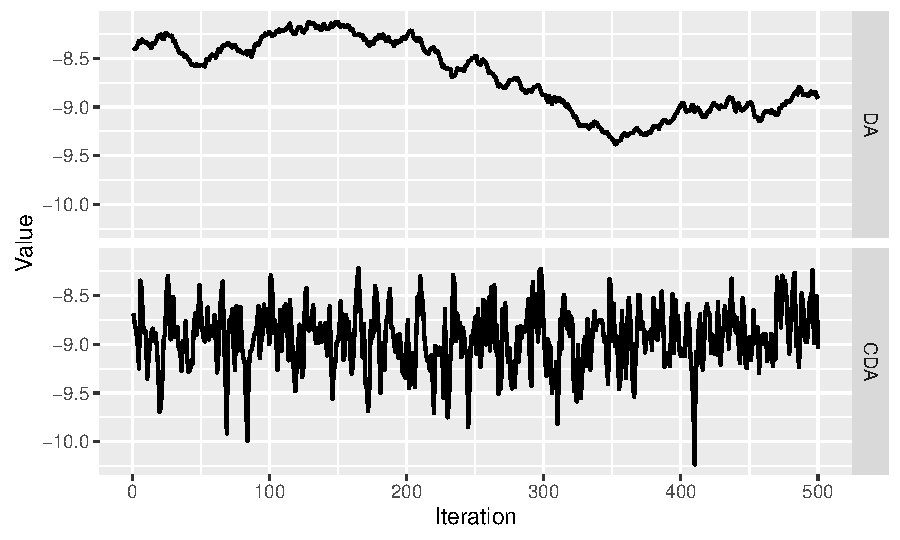
\includegraphics[width=1\textwidth]{logit_random_trace_plot.pdf}
  \caption{Traceplot illustrating mixing performance of the original DA and CDA algorithms in mixed effects logistic regression.}
\end{subfigure}
  \hfill
   \begin{subfigure}[b]{0.49\textwidth}
 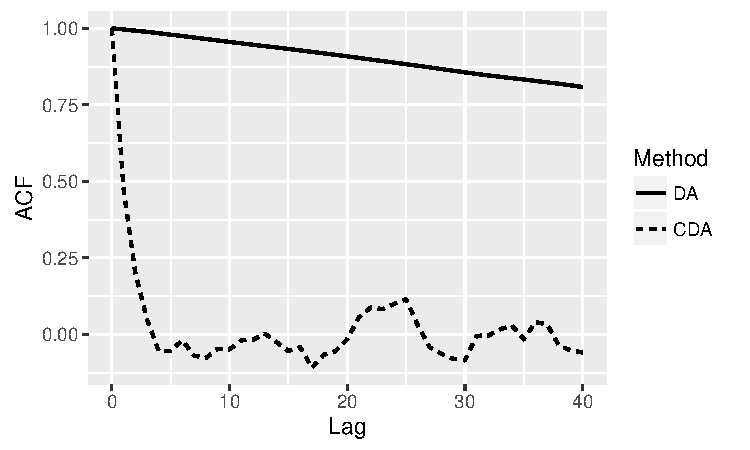
\includegraphics[width=1\textwidth]{logit_random_acf.pdf}
  \caption{Autocorrelation function (ACF) illustrating mixing performance ofthe original DA and CDA algorithms in mixed effects logistic regression.}
\end{subfigure}
 \caption{Panel (a) demonstrates mixing and panel (b) compares marginal and conditional variances for calibrated  \cite{albert1993bayesian} in rare binary data case.}
    \label{logit_random_mixing}
 \end{figure}
 
\section{Theory}

%The strategy of CDA is general and widely applicable. In this section, we present more details. First the reason for accelerated mixing is shown. Then we consider a more general case that involves non-zero approximation error. The error is measured by the total variation distance, which can be controlled via an adaptive strategy with ergodicity guarantee. Lastly, a special case of regression in considered, where the strict bound on the total error can be further relaxed to an individual bound on the likelihood of each data point. A logistic regression model is used to illustrate those results.

\subsection{Mixing Accelaration}

The mixing of Markov chain is related to its geometric convergence rate. Let $\mathcal{P}(\theta,.)$ be the the Markov transition kernel and $\pi(.)$ be its stationary density and $\theta$ be the state in the state space $\varTheta$. The chain is geometrically ergodic if there exist $M: \mathcal{X} \rightarrow [0, \infty)$ and $\rho\in[0,1)$ such that $\delta\{\mathcal{P}^k(\theta,.),\pi(.) \} \le M(\theta^{(0)}) \rho^k$, where $\delta(.,.)$ is the total variation distance $\delta( P_1, P_2) = \underset{\mathcal A\in \mathcal F}\sup ||P_1(\mathcal A)-P_2(\mathcal A)||$.

Consider a space $L^2(\pi)=\{s(\theta): E\{s(\theta)\}=0, var\{s(\theta)\}<\infty \}$. The forward operator $\bf{F}$ can be defined as ${\bf F}s(\theta)=\int P(\theta,\theta') s(\theta') d\theta' = E\{ s(\theta') | \theta \}$, whose norm is equal to the maximal correlation between two states $||{\bf F}||=\underset{s(\theta),t(\theta)\in L^2(\pi)}{\sup}\;\mbox{corr}(s(\theta),t(\theta^{'}))$ \citep{liu2008monte}. This norm is directly related to the convergence rate $\rho$: when the chain is reversible (e.g. Metropolis-Hastings), $\lim_{k\rightarrow \infty}||{\bf F}^k||^{1/k}=\rho$; when the chain is non-reversible (e.g. Gibbs sampling), $||{\bf F}||^2$ is equal to the convergence rate of the reversibilized chain \citep{fill1991eigenvalue}.

The two calibrating strategies proposed above reduce the operator norm.

\begin{theorem}
Let $F$ and $F_{MS}$ be the operators corresponding to the standard DA and the calibrated DA modified with marginalization and sampling (MS), then $||F_{MS}||\le ||F||$.
\end{theorem}


\begin{theorem}
Let $F$ and $F_{IV}$ be the operators corresponding to the standard DA and the calibrated DA modified with increased variance (IV). If the relative difference in marginal variance $\frac{|\mbox{var}\{s(\theta)|y  \} - \mbox{var}_{IV}\{s(\theta)|y\} |}{\mbox{var}\{s(\theta)|y \} }\le \epsilon$ and the variance increase $\frac{ var_{IV}\{ \theta|z,y\}}{ var\{ \theta|z,y\}} \ge (1+\epsilon) $, then $||F_{IV}||\le ||F||$.
\end{theorem}

\subsection{Approximation Error Control in Variance Increased CDA}

For CDA with increased variance, the error needs to be carefully controlled when approximation is involved. We first focus on bounding the total variation distance $||\mathcal{P},\mathcal{P}_r ||_{TV}= \underset{\mathcal A\in \mathcal F}\sup ||\mathcal{P}(\mathcal A)-\mathcal{P}_r(\mathcal A)||$, where $\mathcal{P}$ and $\mathcal{P}_r$ are the measures for the stationary distributions corresponding to the exact and approximate algorithms. From this bound, one can control the errors of the posterior mean and variance.

\begin{theorem}
Let $\theta$ be the $p$-element vector of $\{\theta_j\}_{j=1\ldots p}$.
If the total variation distance between the two measures defined as above is small $||\mathcal{P},\mathcal{P}_r ||_{TV}\le \epsilon_1$, $\pi(\theta|y)$ and $\pi_r(\theta|y)$ have the tail square integral negligible when $|\theta|>M$,  $\mathbb{E} \theta_j^2 {1}_{|\theta_j|>M}\le \epsilon_2$ and $\mathbb{E}_{r} \theta_j^2 {1}_{|\theta_j|>M}\le \epsilon_2$. Let $M$ be large enough so that $\epsilon_2=o(\epsilon_1)$, then the approximation errors between the first two central moments of $\theta_j$ have:
$$|\mbox{E}(\theta_j|y)-\mbox{E}_r(\theta_j|y)|\le M\epsilon_1+ o(\epsilon_1),$$
$$|\mbox{var}(\theta_j|y)-\mbox{var}_r(\theta_j|y)|\le 3M^2\epsilon_1+o(\epsilon_1).$$
\end{theorem}
 
The assumption on the tail is guaranteed by the existence of the second moment, which implies uniform integrablity. The bound on the variance difference is particularly useful in guaranteeing the average increased conditional variable could at most exceed the target variance by a small error $\mathbb{E}^z\mbox{var}_r(\theta_j|z,y)\le\mbox{var}(\theta_j|y)+\epsilon$, with $\epsilon$ as a polynomial function of $\epsilon_1$ defined as above. The approximation error for covariance can be similiarly bounded:

\begin{corollary}
If $\delta( P,P_r)\le \epsilon_1$ and $\pi(\theta|y)$ and $\pi_r(\theta|y)$, $\mathbb{E} \theta_j^2 {1}_{|\theta_j|>M_j}\le \epsilon_2$ and $\mathbb{E}_{r} \theta_j^2 {1}_{|\theta_j|>M_j}\le \epsilon_2$ for $j_1$ and $j_2$.  Let $M_j$ be large enough so that $\epsilon_2=o(\epsilon_1)$, then the approximation error between the covariances:
$$|\mbox{cov}(\theta_{j_1},\theta_{j_2}|y)-\mbox{cov}_r(\theta_{j_1},\theta_{j_2}|y)|\le 3M_{j_1}M_{j_2}\epsilon_1+o(\epsilon_1 ).$$
\end{corollary}

Specifically in regression where the regression coefficient $\beta$ is the focus, the log-distance between the two posteriors is therefore $\log \frac{\pi_{r}( \beta | y,X)}{\pi( \beta | y,X)}=\sum_i^{n}\log \frac{L_{r_i}( y_i| \xbeta)}{L( y_i| \xbeta)}$. As $n$ can be substantially large compared to $p$ and $\{X_i\beta\}_{i=1\ldots n}$ are correlated to each other, it is wasteful to bound the total log distance by a small error. We show under some  mild conditions of the predictor matrix, one can focus on bounding the maximum error from the individual likelihood $\pi(y_i|x_i^T\beta)$ over $i=1\ldots n$ and still obtain the low errors in the first two central moments of $\beta$.

\begin{theorem}
If $x^Tx$ is full rank and let $x^{-}:=(x^Tx)^{-1}x^T$, the following inequalities hold:\\
$$||{E}\beta-{E}\beta_r||_1 \le ||x^{-}||_1 ||{E}x\beta- {E}x\beta_r||_\infty$$
$$||\mbox{cov}\beta-\mbox{cov}\beta_r||_1 \le ||x^{-}||_1 ||x^{-}||_\infty ||\mbox{cov} x\beta- \mbox{cov}x\beta_r||_\infty$$
\end{theorem}

The motivation for using these inequalities is that the norms $||x^{-}||_1$ and $||x^{-}||_\infty$ are quite small, so that bounding the individual errors on the first two moments of $x_i\beta$ is sufficient. For example, when $X$ has each column centered and normalized to unit $1$ and combined with an vector of $\boldsymbol 1$ for intercept, then $||x^{-}||_\infty\approx 1/n$ and $||x^{-}||_1\approx p$. One would expect with $n$ large and $p$ moderate, bounding the error in $\epsilon/p$ on $||\mathbb{E}x\beta- \mathbb{E}x\beta_r||_\infty$ and $\epsilon n/p$ on $||\mbox{cov} x\beta- \mbox{cov}x\beta_r||_\infty$ is enough to have near optimal result. These results also apply to the over-dispersed model where each $\xbeta$ is replaced by $\eta_i=  \xbeta + \gamma_i$ with $\gamma_i\sim N(0,\sigma^2)$. For more complex setting such as random effects $\{ s_i\gamma_i\}_{i=1\ldots n} \sim \mathcal{N}(0,\Sigma)$, one can revert to bound the total distance $\log \frac{\pi_{r}( \beta | y,X)}{\pi( \beta | y,X)}$ for simpler control.


We return to examine the CDA for mixed effects logistic regression here.

{\bf Calibration Example 3 (continued): Mixed Effects Logistic Regression}

In the CDA for mixed effects logistic regression, the effective approximate likelihood is $L_{r}(y_i|\eta_i) = \frac{\Gamma(1/r_i+1)}{\Gamma(y_i+1)\Gamma(1/r_i-y_i+1)}\frac{\exp (\eta_i+ \log r_i)^ {y_i}}{\{1+\exp (\eta_i+ \log r_i)\}^{1/r_i}}$. The distance between the approximate and the true likelihoods for each $i$ has $|| { L_{r}(y_i|\eta_i) } - {L(y_i|\eta_i)} )||_{TV} \le   \{   \frac{\sqrt{r_i-1}  \exp(\eta_i)}{2} \} 1 \{\eta_i< - \log r_i \le 0 \}$. The tail integral $E \eta^2_i 1(|\eta_i|>M) = O\{ M^2 \exp(-M)\}$. 

Given the maximally tolerable approximation error $\epsilon$ for $||\mathbb{E}\beta-\mathbb{E}\beta_r||_1$ and $||\mbox{cov}\beta-\mbox{cov}\beta_r||_1$, the choice for truncation $M: M^3 \exp(-M) < \frac{\epsilon}{3M  ||x^{-}||_1 ||x^{-}||_\infty || \vee ||x^{-}||_1 }$, and then the working parameter $r_i \le \frac{ 4 \epsilon^2 \exp(-2\eta_i)}{(3M^2  ||x^{-}||_1 ||x^{-}||_\infty || \vee M ||x^{-}||_1 )^2} $ if $r_i>1$ can hold, otherwise $r_i$ is set to $1$ to eliminate the error. Using the simulation setting as the numerical example, $||x^{-}||_\infty =6 \cdot 10^{-5}$ and $||x^{-}||_1 =1.96$, given $\epsilon=0.01$, $M=15$ satisfies the error bound. This leads to approximately $r_i \le  [\{\frac{10^{-3} }{\exp(\eta_i)}\}^2  \wedge {\exp(-\eta_i)} ]  \vee 1$. This suggests applying calibration when $\eta_i< -6.9$ approximately, which is consistent with the rare event scenario.

\subsection{Ergodicity}

The conditions for ergodicity should be met for Markov chains. In the CDA based on marginalization, obviously as long the original chain is ergodic, so is the marginalized chain is, due to its smaller norm of the forward operator. For the CDA based on variance increase, the adaption of the working parameters could influence the ergodicity. In the numerical solution, we stop adaption after the tuning period; in the analytical solution, we rely on the the results from \cite{roberts2007coupling} that an adaptive Markov chain is uniformly ergodic, if (i) the transition kernel corresponding to each $r$ is uniformly ergodicity (simultaneous convergence) and (ii) the total variation distance between kernels in two adjacent steps converges to $0$ in probability (diminishing adaptation).

The first condition is simple to achieve since the approximation does not alter the distribution of the transition kernel but only with different parameterization, the condition can be met with only slight modification. For the diminishing adaptation, we let each $r_i$  be  the extreme function of the value in $\varTheta^*$. As most of the extreme function converge in probability. The convergence of $r$ hence leads to the convergence of the transition kernel by continuous mapping theorem.

{\bf Calibration Example 3 (continued): Mixed Effects Logistic Regression}

In the CDA with mixed effects logistic regression, we set $r_i =  1 \vee \underset{\eta_i: \theta\in \varTheta^*}{\inf}[\{\frac{10^{-3} }{\exp(\eta_i)}\}^2  \wedge {\exp(-\eta_i)} ]   $, which is related to the maximum of $\eta_i=\xbeta+z_i\gamma_i$ if $\eta_i<0$. With finite variance of $\beta$ and $\gamma_i$, the value is convergent in probability via Chebyshev's inequality. The diminishing adaption for the numeric example is shown in Figure~\ref{diminishing_adapt}.

 \begin{figure}[H]
 \centering
 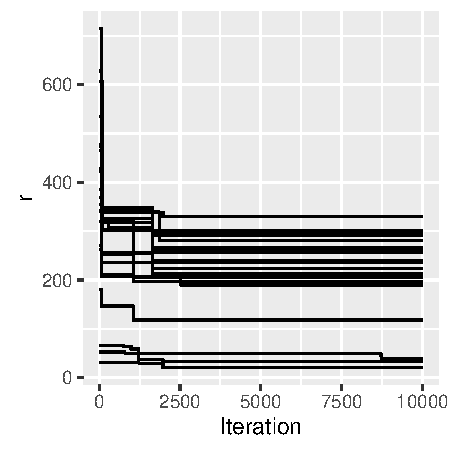
\includegraphics[width=0.3\textwidth]{r_adaptation.pdf}
  \caption{The diminishing adaptation of the working parameter $r_i$.}
  \label{diminishing_adapt}
 \end{figure}

\section{Real Data Application: Poisson Regression for Online Advertisement Tracking}

We now apply CDA to a large data application in online advertisement tracking. The dataset contains the click-through count between pairs of website. There are $n=59,792$ originating websites, where the advertisement is displayed, and $96$ different target websites where the link points to. The training data is collected during a two-week period, the a non-overlapping set is collected during another two-week time for testing purpose. For a given website, it is of commercial interests to predict the traffic from each originating one $y_i$, using the information from the other $p=95$ websites $x_{i,1},\ldots, x_{i,95}$. Therefore, this leads to a count regression model.

Due to its large number of the originating websites, not every link produces traffic to the target. As the result, the outcome data is inflated with $0$'s and  only $4.5\%$ contains count greater or equal to 1. For this zero-inflated scenario, Poisson log-linear model is known for slow mixing in Metropolis-Hastings algorithm. Despite that zero-inflated model is widely favored for its explanation of $0$'s, it does not solve the slow mixing issue.  Due to high correlation of $\pi_i$ and the Poisson mean, the mixing can be even slower (see appendix for autocorrelation from zero-inflated Poisson model with Metropolis-Hastings). Moreover, for prediction purpose, it would be important to predict if the outcome is zero via the predictors, leading to more complicated model such as $y_i\sim \pi_i(g(X_i^T\beta_1))  1_{y_i=0}+ \{ 1-\pi_i(g(X_i^T\beta_1)) \} Poisson\{\exp (X_i^T \beta_2)\}$.

Rather, we consider calibrating the simple model $y_i\sim Poisson\{\exp(X_i^T\beta)\}$ for $i=1\ldots n$. As it contains a quite negative intercept, a large proportion of the prediction would have the mean close to $0$. At the same time, a small proportion can deviate from $0$ as the predictors differ from the majority. This would achieve the same goal as the predictor-based zero-inflated model, but is much more tractable for computation. Obviously, the success of this model would rely on a rapid convergence and good mixing in Markov chain, so that the parameters can be accurately estimated with good uncertainty quantification.

{\bf Calibration Example 4: Poisson Log-Linear Regression with Zero-Inflated Data}

We now derive a CDA for Poisson log-linear regression. Although the normal approximation are proposed for large Poisson mean, it can be awkward for small count data. \cite{zhou2012lognormal} used negative binomial $\mathcal{NB}\{ \alpha,\frac{\exp(X_i^T\beta)}{\exp(X_i^T\beta)+\alpha}\}$ with large $\alpha$ as an approximation. Instead, we utilize a simpler limit form based on $\pi(y_i|X_i,\beta)=\frac{ \exp(y_i X_i^T\beta)}{\exp\{\exp(X_i^T\beta)\}y!} =\lim_{\lambda\rightarrow\infty}\frac{\exp(y_i X_i^T\beta)}{\{1+ \exp(X_i^T\beta)/\lambda\}^{\lambda}y!}$. The new form enables Polya-Gamma augmentation $ \pi(y_i|X_i,\beta) \propto \exp\{(y_i-\lambda/2)(X_i^T\beta-\log \lambda)\}\int exp(- \frac{z_i (X_i^T\beta-\log \lambda)^2}{2})\mathcal{PG}(z_i|\lambda, 0)d z_i$ for each $i$. With large $\lambda$ approximation, the posterior is sample by updating individual $z_i$ from $\mathcal{PG}\left\{\lambda, X_i^T\beta-\log \lambda\right\}$ and $\beta$ from $\mathcal{N}\big[ (X^T \Omega X )^{-1} (X^T  \big \{ y - \lambda/2 + z \log \lambda \big\} ),(X^T \Omega X )^{-1} \big]$ where $\Omega=diag\{z_i\}$, based on a flat prior on $\beta$.

However, the mixing is inherently slow, due to the large $\lambda$ approximation affecting large $\Omega$, hence small $\mbox{var}(\beta|z,y,X)=(X^T \Omega X )^{-1}$. We calibrate this issue by simply replacing the global large $\lambda$ with individual small value $\tau_i=1/r_i>0$. The integration leads to $\pi_{r_i} (y_i| X_i^T \beta) =\frac{\Gamma(1/r_i+1)}{\Gamma(1/r_i-y+1)\Gamma(y+1)}\frac{\exp ( X_i^T\beta+\log r_i)^y_i}{\{1+ \exp ( X_i^T\beta+\log r_i)\}^{1/r_i}}$ with $y_i-1<1/r_i$. We left the approximation error calculation and choice for $r_i$ in the appendix.

To obtain results, we ran DA with large $\lambda=10,000$, CDA and Hamiltonian Monte Carlo (HMC) for posterior computation. We started all three algorithms by assigning the same initial value $(X^TX)^{-1}(X^T log( y+1))$ to ${\beta}$. We ran DA for $4000$ steps due its extremly slow convergence after $2000$ iterations; HMC for $2,000$ steps;  CDA for $2,000$ as it quickly converged in the first $50$ iterations. We use the last $1,000$ as posterior samples for all three. 

The mixing of DA and CDA is compared by traceplots and autocorrelation plots in Figure~\ref{data_poisson}. DA shows slow mixing for several parameters (Figure\ref{acf_poi_da}), including the important intercept estimate $\beta_0$ (first plot in Figure\ref{traceplot_poi_da}). In contrast, CDA performs extremely very well in terms of mixing (Figure\ref{acf_poi_ada}). This is shown by the low autocorrelation in all of the $96$ parameters. 

 \begin{figure}[H]
 % \centering
   \begin{subfigure}[b]{0.45\textwidth}
 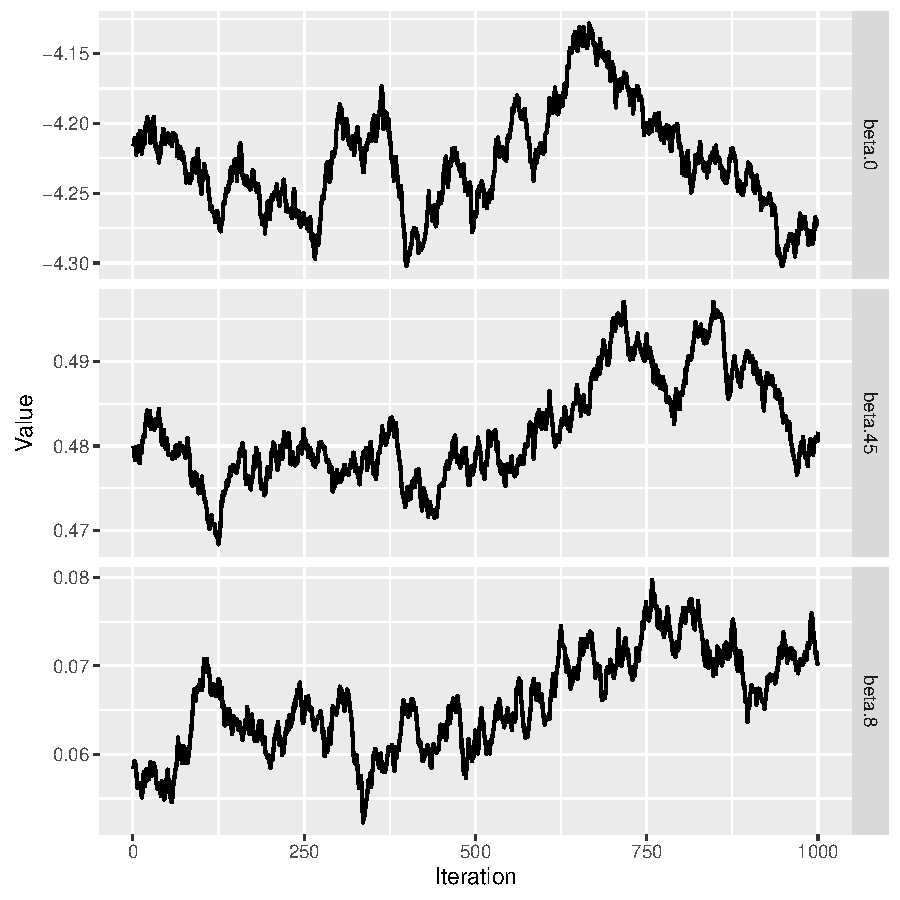
\includegraphics[width=1\textwidth]{traceplot_poisson_da.pdf}
 \caption{Trace plots of three parameters from DA.}
  \label{traceplot_poi_da}
 \end{subfigure}
  \hfill 
 \begin{subfigure}[b]{0.45\textwidth}
 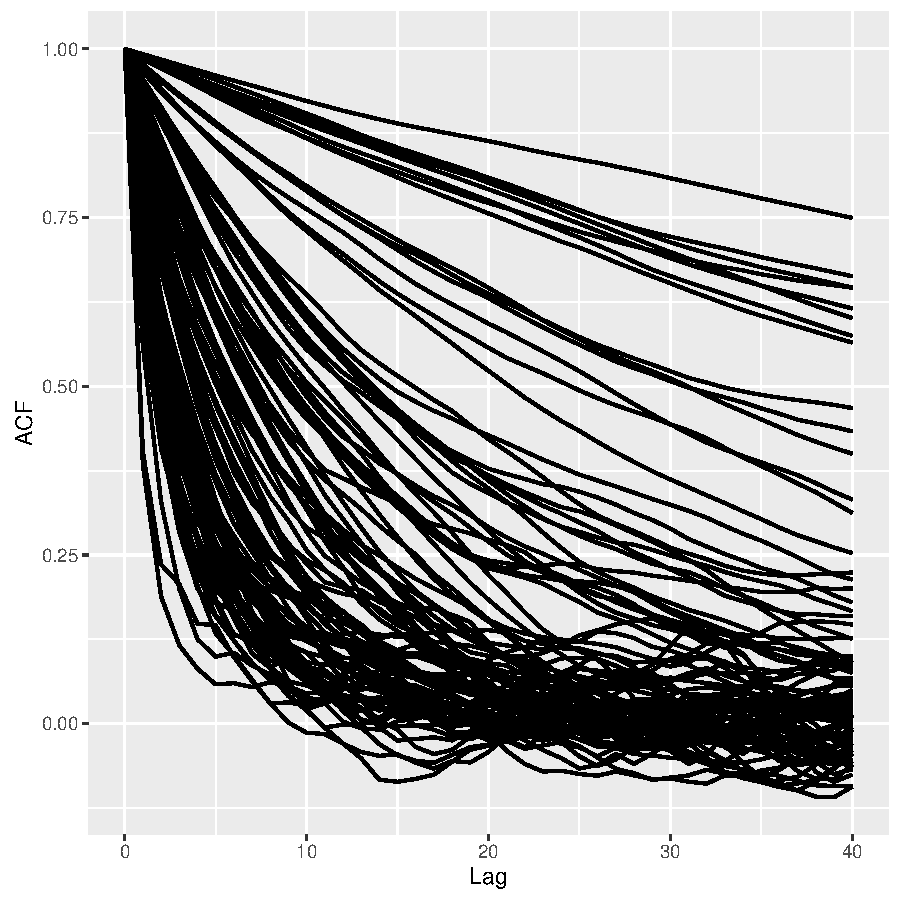
\includegraphics[width=1\textwidth]{poisson_da_acf.pdf}
 \caption{Autocorrelation of all the 96 $\beta$'s from DA.}
   \label{acf_poi_da}
 \end{subfigure} 
  \begin{subfigure}[b]{0.45\textwidth}
 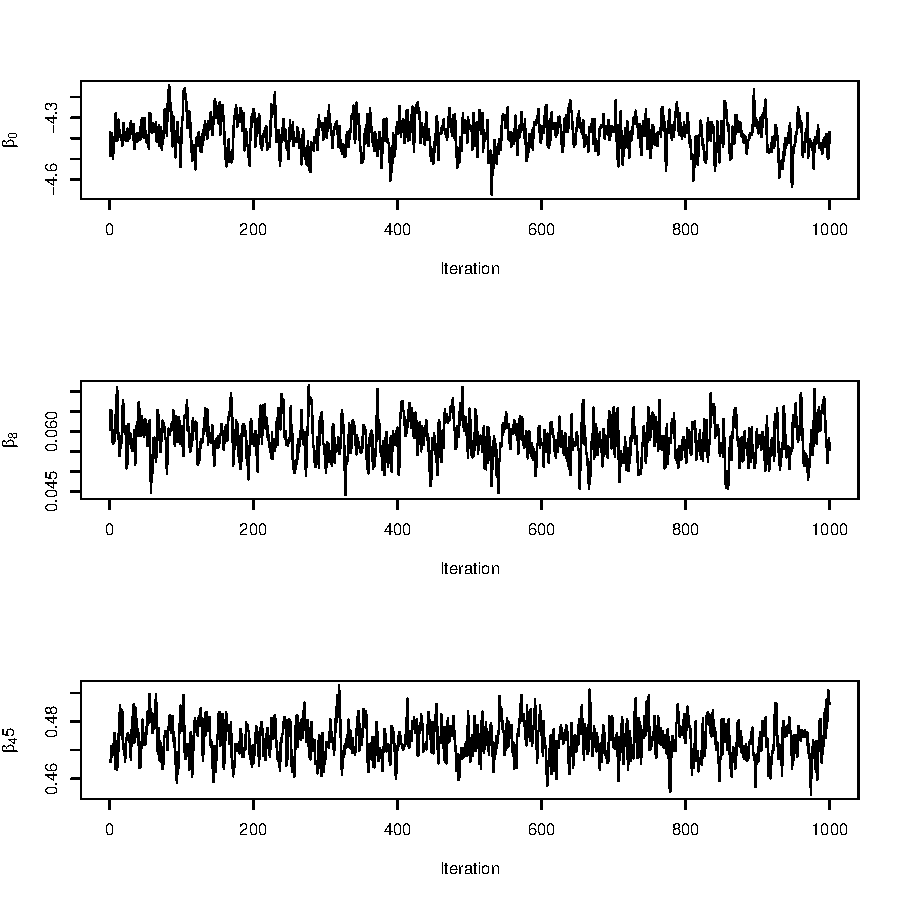
\includegraphics[width=1\textwidth]{traceplot_poisson_ada.pdf}
 \caption{Trace plots of three parameters from CDA.}
  \label{traceplot_poi_ada}
 \end{subfigure}
  \hfill 
 \begin{subfigure}[b]{0.45\textwidth}
 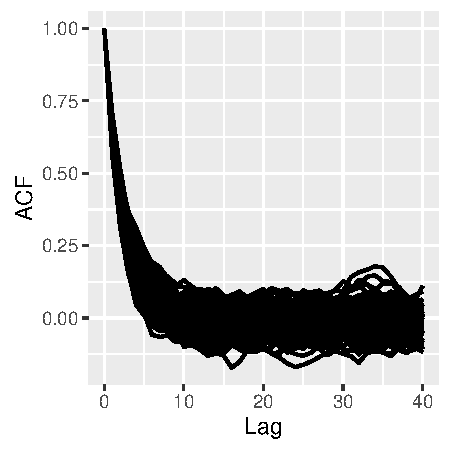
\includegraphics[width=1\textwidth]{poisson_ada_acf.pdf}
 \caption{Autocorrelation of all the 96 $\beta$'s from CDA.}
   \label{acf_poi_ada}
 \end{subfigure}
 \caption{Compared with DA, CDA produces much faster mixing posterior sample.}
 \label{data_poisson}
 \end{figure}



We list the parameter estimates and fit statistics in Table~\ref{table:Poisson}. For simplicity, we include the posterior mean and standard deviation for the intercept $\beta_0$ and the sum of slopes $\sum_{j=1}^{95} \beta_j$. To assess goodness-of-fit, we also evaluate root-mean-squared error $RMSE= \sqrt{ \sum_{i=1}^n  (y_i-\mu_i)^2/n}$ and the deviance $D=2\sum_{i=1}^n \{ y_i \log(y_i/\mu_i)  1_{y_i>0} -(y_i-\mu_i)\}$, with $\mu_i=\exp( X_i{\hat\beta})$ and ${\hat\beta}$ is the posterior mean. For prediction performance, we use the testing dataset collected $\{ y_{new},  X_{new}\}$ on the same websites and $\tilde y_{i,new}=\exp( X_{i,new}{\hat\beta})$ as the estimator. We evaluate the cross-validation RMSE between $y_{i,new}$ and $\tilde y_{i,new}$.

As expected, the estimate for $\beta_0$ is quite negative, which is captured by the point estimates of both DA and CDA. However, the slow mixing DA underestimates the variance of the intercept. The estimates for the $95$ covariates differ greatly between the CDA and DA. Obviously, the poor mixing leads to Markov chain trapped in a suboptimal fit to the data, whereas CDA performs exceptionally well in fit statistics and the validation error that is almost 4 times lower. The details in comparing the fitted and prediction are provided in the appendix.

To verify the result, we also use HMC as the reference. HMC is known for its good mixing properties but very costly evaluation . The result of CDA agrees very well with HMC in both the posterior mean and standard deviation on all the $95$ slope parameters (see appendix for comparison plots). For HMC, it requires significant tuning to reach ideal step size and length for proposal; while CDA only require one additional  step in generating the latent variable. Therefore, CDA is significantly more efficient than HMC and took only $1/10$ of the computing time.


\begin{table}[H]
\centering
\begin{tabular}{|l |r |r| r| r |} 
 \hline
                          & DA & CDA & HMC\\
 [0.5ex]
 \hline
$\beta_0$                         & -4.21 (0.042)& -4.38 (0.075) & -4.47 (0.071) \\
$\sum_{j=1}^{95} \beta_j$         & -0.11 (0.063)& 0.69 (0.053)  & 0.70 (0.055)  \\
RMSE                              & 32.86        & 5.06          & 4.88\\
D                                 & 182127.7     & 107076.9      & 106791.3\\
CV-RMSE                           & 32.01        & 8.61          & 8.28\\
Steps to Converge                 & 2000         & 50            & 500 \\
Computing Time (per 2,000 steps)  & 50 mins       & 51 mins        & 600 mins\\
 \hline
\end{tabular}
\caption{Performance of DA, CDA and HMC in Poisson regression with online advertisement tracking data. Posterior estimates for the intercept and sum-of-slopes are shown. The CDA shows much better fit statistics such as root-mean-squared error (RMSE) and deviance (D). In cross-validation (CV-RMSE), the CDA outperforms DA as well. The CDA converges much more rapidly than DA. Compared to the reference, CDA agrees with the HMC very well but takes significantly less time.}
\label{table:Poisson}
\end{table}


\section{Discussion}

The slow mixing is a severe problem that prevents data augmentation based MCMC from be applicable on large dataset. With data size increases and become complex, it is common for the parameters to deviate from the usual area with reasonable mixing performance. As we show in the previous example, it does not only lead to an unmanagable increase in the computational time, but also results in Markov chain trapped in the suboptimal state.  Therefore, it is necessary to address this issue if we want to keep data augmentation useful in large data.

In this article, we propose a solution that calibrates the conditional variance of the parameter onto the same order of the marginal variance, and therefore significantly accelerate the mixing and convergence. The approach is general and simple to apply in most of the existing data augmentation methods. We expect it can be used in more sophisticated models as well, such as hierarchical or random effect models.

 We use Hamiltonian Monte Carlo as a good reference for parameter estimation. Here we give a brief comparison between CDA and HMC.  The ideal Markov chain kernel  would be to propose, based on the current state, a state that is as uncorrelated as possible; in the meantime, with high acceptance probability to move to the new state. The HMC utilizes numerical simulation of Hamiltonian dynamics and a long walk to generate such a proposal. In contrast, the CDA directly utilizes the original density but with an increased conditional variance to reduce the correlation. The  short distance between the proposal and current likelihood  enables a good acceptance rate as well. The difference between the two is that the HMC is computationally costly since it relies on evaluation of gradients and multiple Hamiltonian steps for each proposal; whereas CDA does not use gradient but only one-step update, which is almost at the same low cost as the conventional DA method. 

In this article, we utilize density approximation in the CDA algorithm. As a alternative, the approximation can be always made exact with an additional Metropolis-Hastings step at each iteration. The Metropolis-Hastings enjoys the adaptive nature for optimizing posterior mixing, but is difficult in selecting proposal distribution. This problem becomes obvious when the parameters are multi-dimensional and correlated. The CDA-coupled Metropolis Hastings can be viewed as one solution to this problem, as the proposal from an approximation of the likelihood naturally accommodates the correlation structure and leads to good acceptance rate.


\bibliography{reference}
\bibliographystyle{plainnat}


\section{Appendix}

\subsection{Proof of Theorems}

\subsubsection{Distance between Logistic Regression}
\begin{equation}
\begin{aligned}
\log \frac{ L_{r}(y_i|\eta_i) }{L(y_i|\eta_i)} & =\log \frac{\Gamma(1/r_i+1) r_i^{y_i}  /\Gamma(1/r_i -y_i+1)  }{\Gamma(2) /\Gamma(2 -y_i)  } + \log \frac{ 1+\exp(\eta_i)}{ \{1+\exp(\eta_i)r_i\}^{1/r_i}}\\
& =\log\{1+ \exp ( \eta_i)\}   - 1/r \log\{1+ r\exp ( \eta_i)\}\\
& \le   \{   (r_i-1) \frac{ \exp(2\eta_i)}{2} \}  1\{\exp(\eta_i)< 1/r_i\} + \log \frac{ 1+\exp(\eta_i)}{ \{1+\exp(\eta_i)r_i\}^{1/r_i}}  1\{\exp(\eta_i)\ge 1/r_i\} \\
%& \le   \frac{r_i-1}{2 r_i^2}  1\{r_i <\exp(-\eta_i) \} + \log \frac{ 1+\exp(\eta_i)}{ \{1+\exp(\eta_i)r_i\}^{1/r_i}}  1\{ \eta_i \ge -\log r_i\}.
\end{aligned}
\end{equation}

Using adaptive $r_i$ such that $r_i <\exp(-\eta_i)$ guarantees the Kullback-Leibler distance $KL ( { L_{r}(y_i|\eta_i) } || {L(y_i|\eta_i)} ) \le \frac{r_i-1}{2 r_i^2} $. As $r_i\ge 1$, when $\exp(-\eta_i) < 1$, setting $r_i=1$ leads to $KL ( { L_{r}(y_i|\eta_i) } || {L(y_i|\eta_i)} ) =0 $



as $r_i\ge 1$, For bounding the approximation error, the log-distance has $\log\frac{\pi_{r_i}(\theta|y)}{\pi(\theta|y)} \le     (r-1) \frac{n \exp(2\theta)}{2}   1_{\exp(\theta)< 1/r}$. We assign $r= {\tau}{ \exp(-\theta)} \vee 1$ with $\tau<1$ so that $r$ takes large value when  $\exp(\theta)< 1/r \le 1$, otherwise $r=1$ reduces to exact $\pi(\theta|y)$. The log-distance can be further simplified to $\log\frac{\pi_{r_i}(\theta|y)}{\pi(\theta|y)}\le \tau\frac{n\exp(\theta)}{2}$. In order to have $\delta(P,P_r)\le\epsilon$, it suffices to have $\tau< \frac{4\epsilon^2}{n\exp(\theta)}$.

\subsubsection{Tail Integral in Logistic Regression}

Consider each likelihood $L(y_i|p_i) = p^y_i (1-p)^{1-y_i}$ with $p_i=\frac{\exp(\eta_i)}{1+\exp(\eta_i)}$. Applying density transformation leads to 
$\pi(\eta_i|y_i) = 2\frac{\exp(\eta_i) \exp(y_i\eta_i)}{\{1+\exp(\eta_i)\}^3}$.

If $y_i=1$,
\begin{equation}
	\begin{aligned}
			E\{ \eta_i^2 1(|\eta_i|>M) \} & = E\{ \eta_i^2 1(|\eta_i|>M, \eta_i \ge 0 ) \} + E\{ \eta_i^2 1(|\eta_i|>M, \eta_i<0 ) \} \\
	& \le 2\int_M^{\infty} \frac{\eta_i^2}{1+\exp(\eta_i)} d\eta_i + 2\int_{-\infty}^{-M}{\eta_i^2}{\exp(2\eta_i)}d\eta_i  \\
	& \le 2\int_M^{\infty} {\eta_i^2}{\exp(-\eta_i)} d\eta_i +2 \int_{-\infty}^{-M}{\eta_i^2}{\exp(2\eta_i)}d\eta_i \\
	& = 2(M^2+2M+2)\exp(-M) + \frac{1}{2} (2M^2 + 2M +1) \exp(-2M).
	\end{aligned}
\end{equation}

if $y_i=0$,
\begin{equation}
	\begin{aligned}
			E\{ \eta_i^2 1(|\eta_i|>M) \} & = E\{ \eta_i^2 1(|\eta_i|>M, \eta_i \ge 0 ) \} + E\{ \eta_i^2 1(|\eta_i|>M, \eta_i<0 ) \} \\
	& \le 2\int_M^{\infty} \frac{\eta_i^2}{\{1+\exp(\eta_i)\}^2} d\eta_i + 2\int_{-\infty}^{-M}{\eta_i^2}{\exp(\eta_i)}d\eta_i  \\
	& \le 2\int_M^{\infty} {\eta_i^2}{\exp(-2\eta_i)} d\eta_i +2 \int_{-\infty}^{-M}{\eta_i^2}{\exp(\eta_i)}d\eta_i \\
	& =\frac{1}{2} (2M^2 + 2M +1) \exp(-2M)+  2(M^2+2M+2)\exp(-M) .
	\end{aligned}
\end{equation}

Therefore, letting $M=21$ leads to the tail error $\epsilon_2\le 10^{-6}$.






\subsection{The Numerically Optimized $r_i$'s in Probit CDA}


\begin{figure}[H]
 \centering
 \begin{subfigure}[b]{0.5\textwidth}
 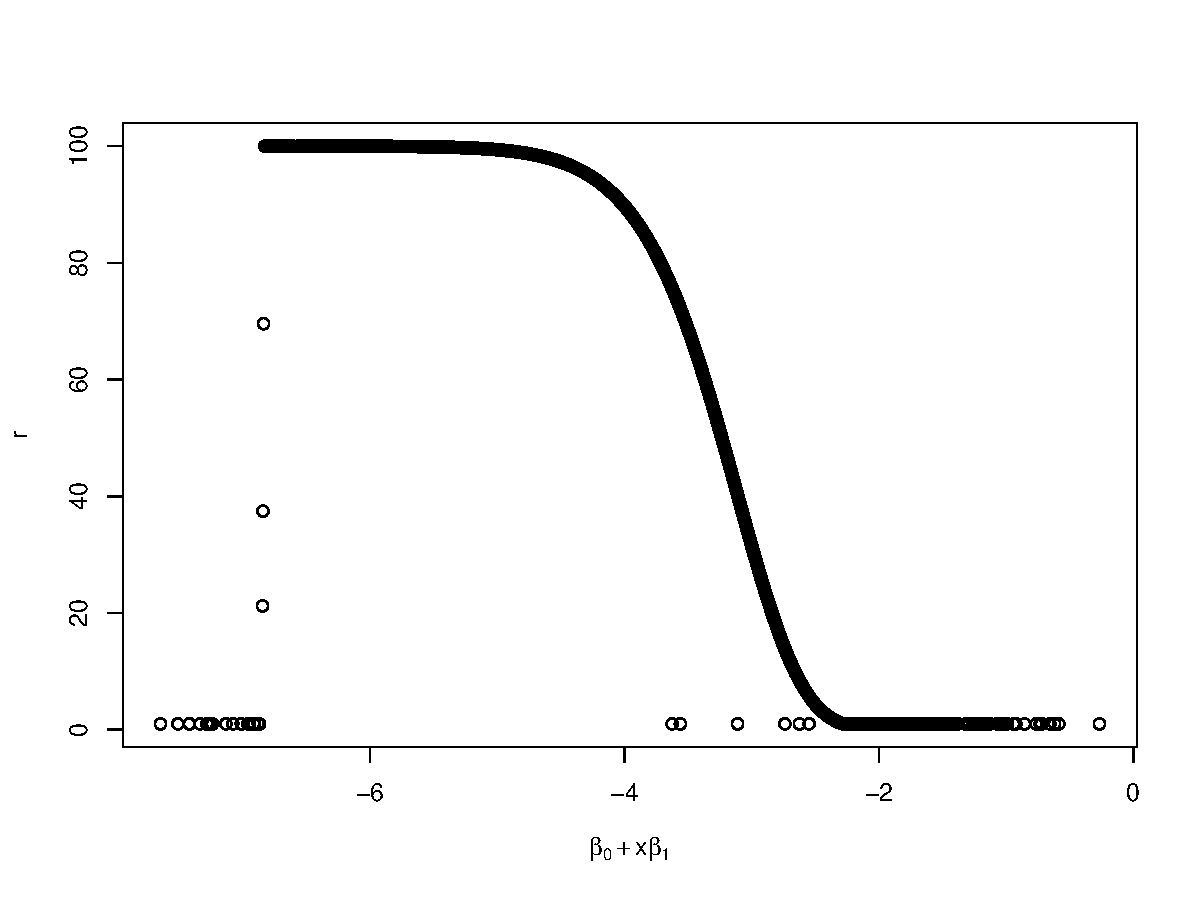
\includegraphics[width=1\textwidth]{probit_ada_r.pdf}
 \caption{$\beta_0=-1, \beta_1=1$}
 \end{subfigure}
 \caption{Numerically learned $r_i$ in probit CDA}
 \end{figure}


\subsection{Mixing of Zero-inflated Poisson using DA}


 \begin{figure}[H]
 % \centering
   \begin{subfigure}[b]{0.45\textwidth}
 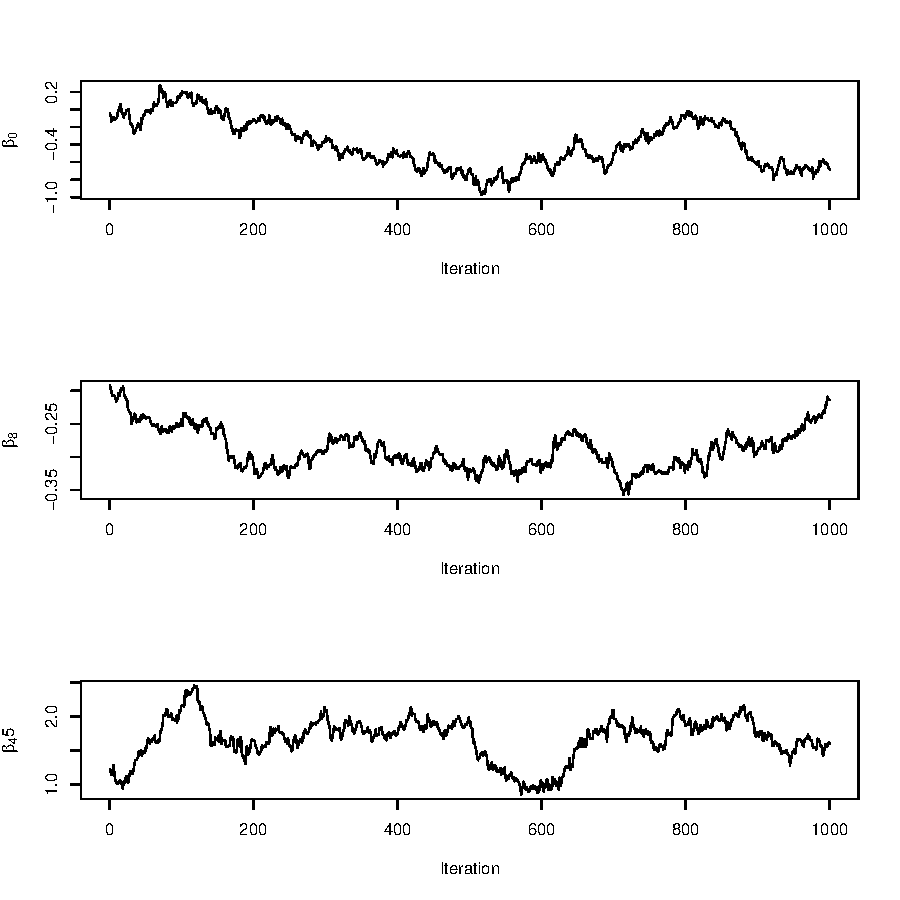
\includegraphics[width=1\textwidth]{traceplot_poisson_zip_da.pdf}
 \caption{Trace plots of three parameters from DA ZIP model}
 \end{subfigure}
  \hfill 
 \begin{subfigure}[b]{0.45\textwidth}
 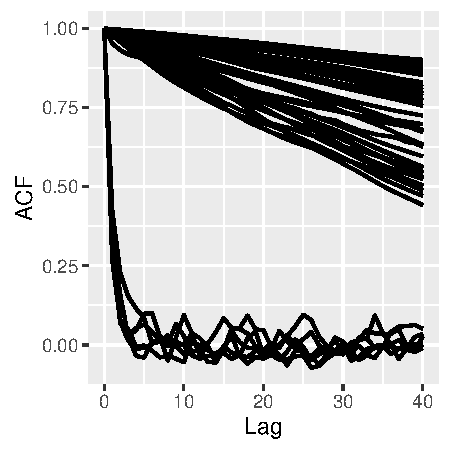
\includegraphics[width=1\textwidth]{poisson_zip_da_acf.pdf}
 \caption{Autocorrelation of all the 96 $\beta$'s from DA ZIP model.}
 \end{subfigure}  
 \caption{The hierarchy in the zero-inflated Poisson model does NOT help reduce the autocorrelation.}
 \end{figure}



\subsection{Goodness-of-Fit and cross-Validation for Poisson Regression}


 \begin{figure}[H]
 % \centering
   \begin{subfigure}[b]{0.45\textwidth}
 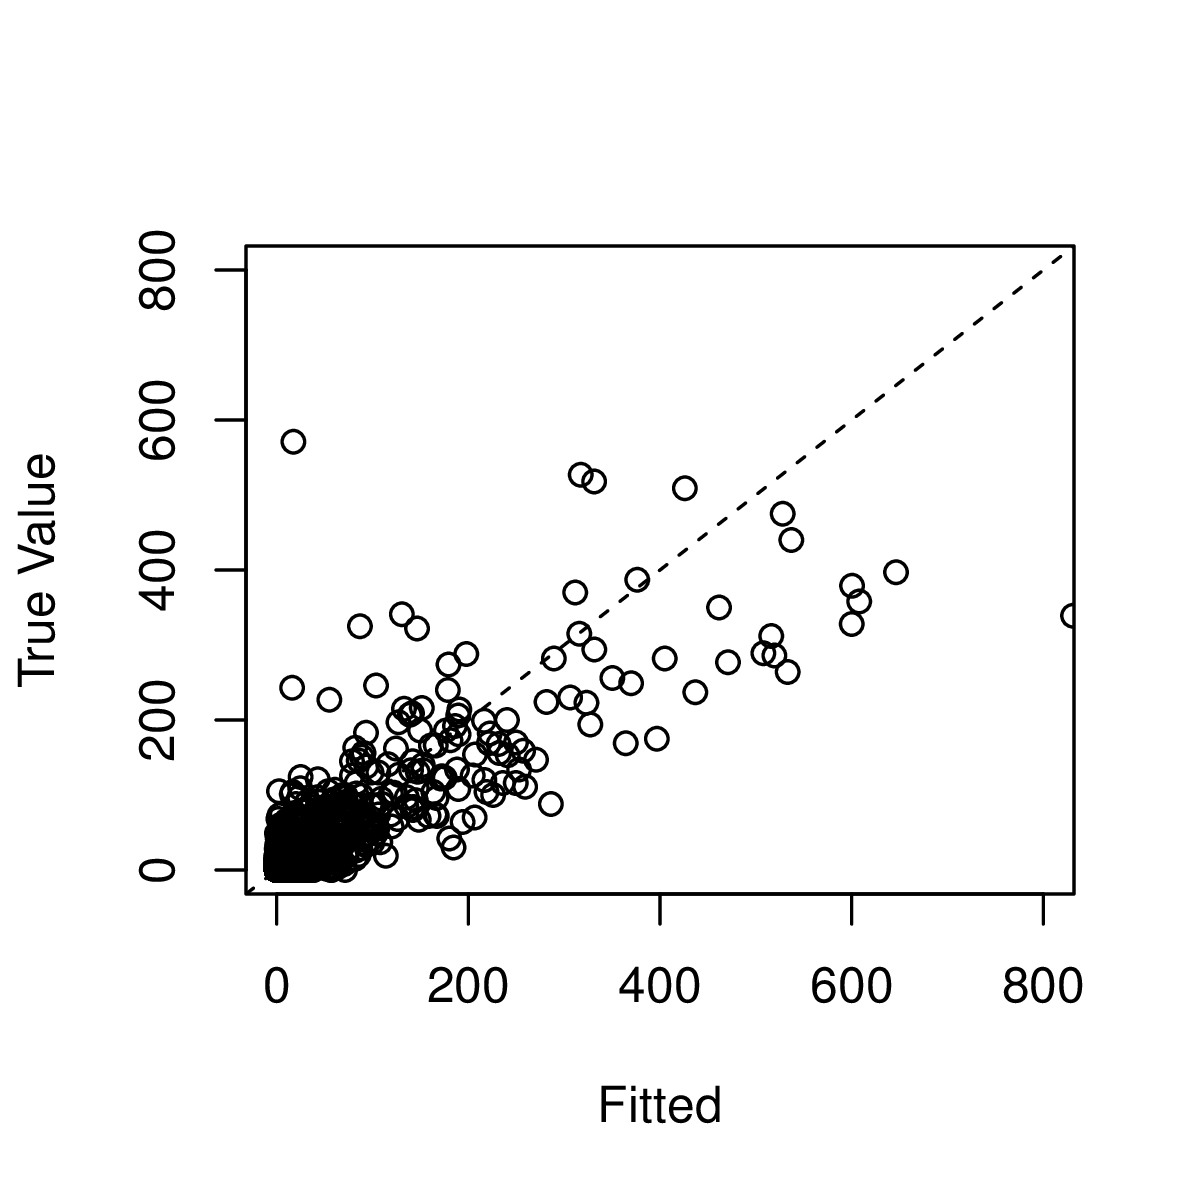
\includegraphics[width=1\textwidth]{poisson_fitting_da.png}
 \caption{Fitted vs true values using DA}
 \end{subfigure}
  \hfill 
 \begin{subfigure}[b]{0.45\textwidth}
 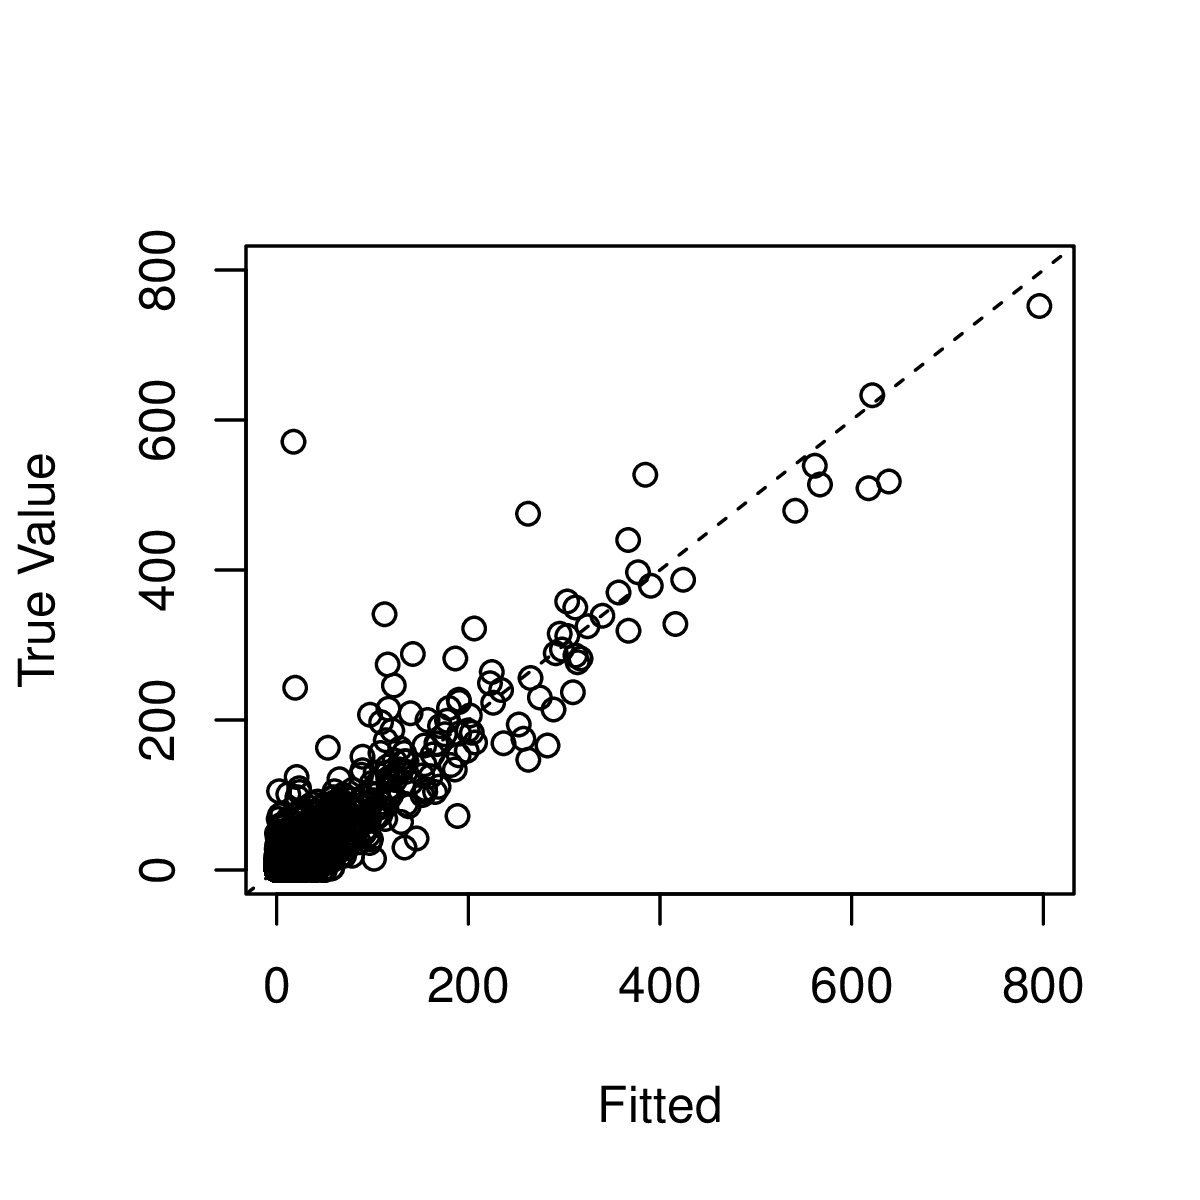
\includegraphics[width=1\textwidth]{poisson_fitting_ada.png}
 \caption{Fitted vs true values using CDA}
 \end{subfigure}  
   \begin{subfigure}[b]{0.45\textwidth}
 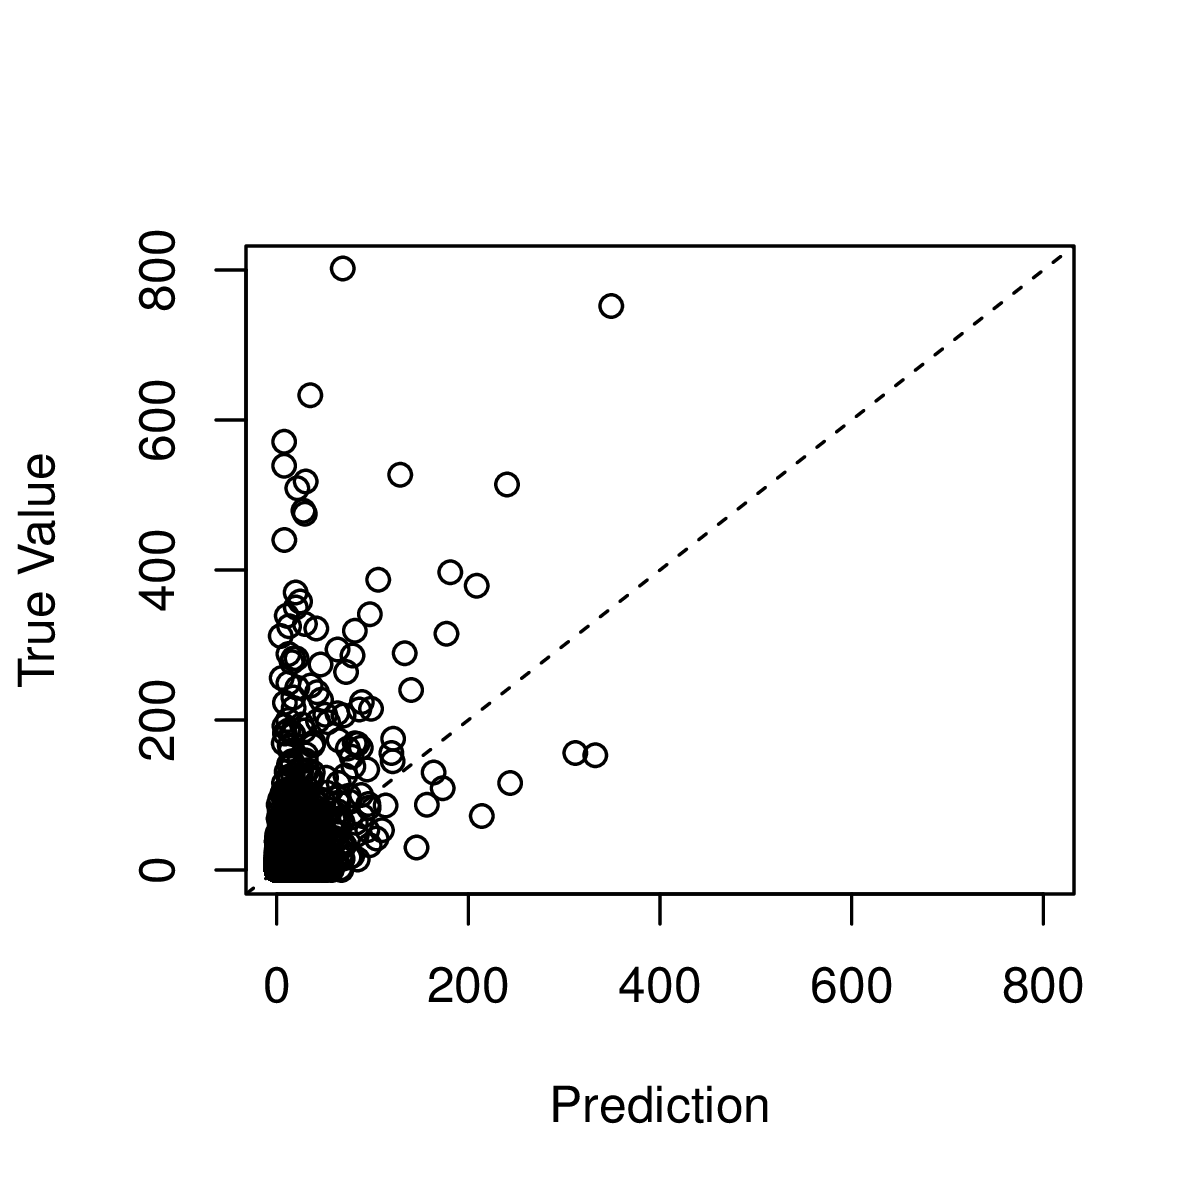
\includegraphics[width=1\textwidth]{poisson_cv_da.png}
 \caption{Prediction vs true values using DA}
 \end{subfigure}
  \hfill 
 \begin{subfigure}[b]{0.45\textwidth}
 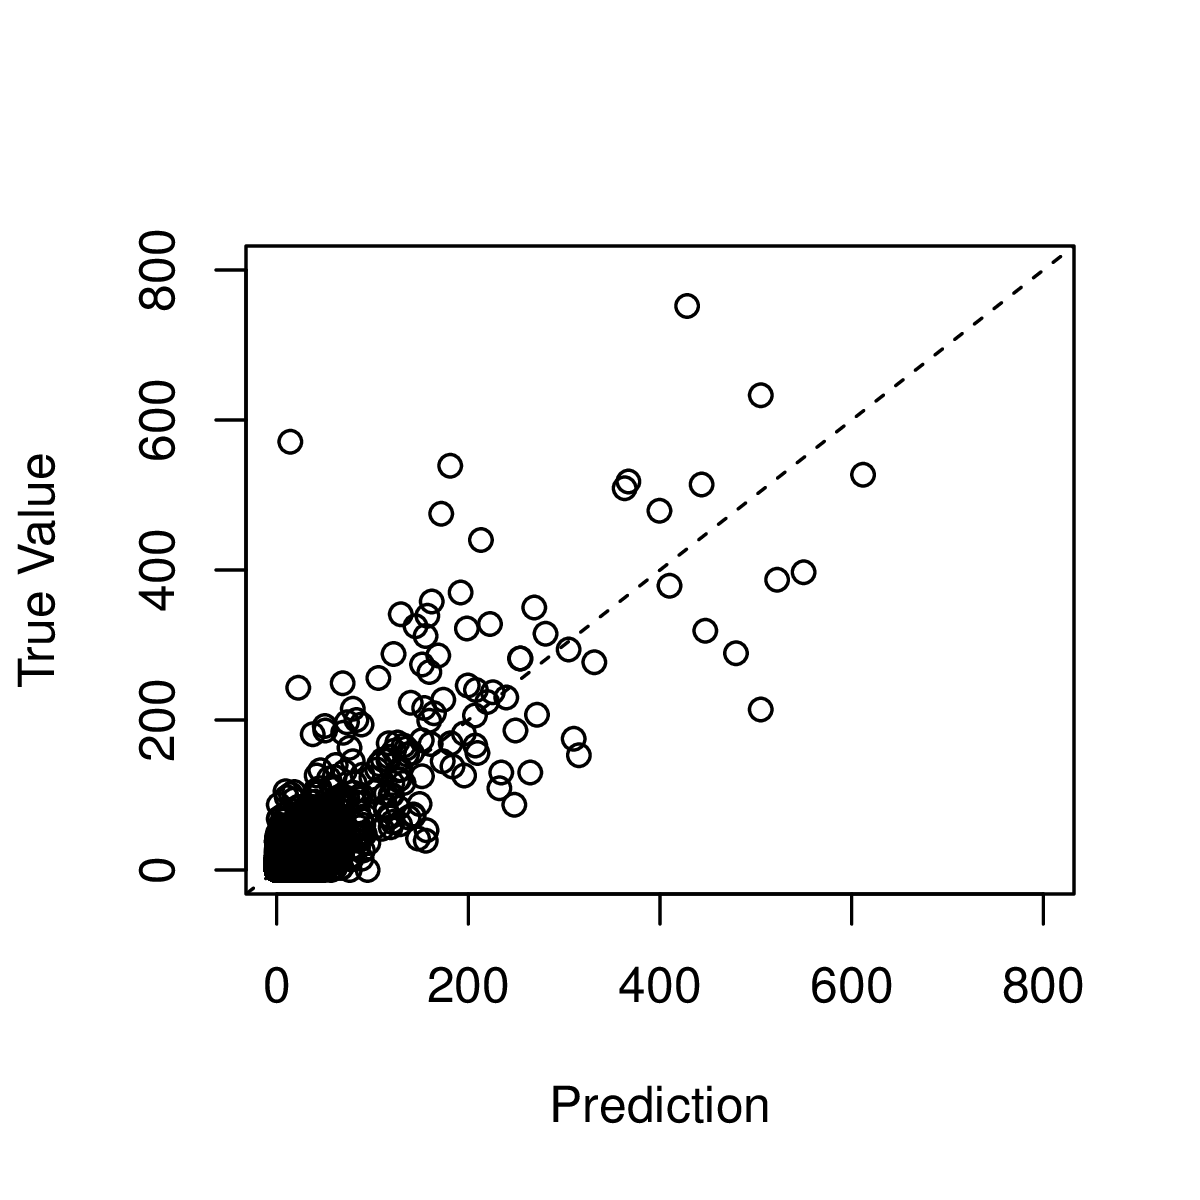
\includegraphics[width=1\textwidth]{poisson_cv_ada.png}
 \caption{Prediction vs true values using CDA}
 \end{subfigure} 
 \caption{The posterior estimates produced by CDA is better fitted to the data and have more accurate prediction than DA.}
 \end{figure}

 \subsection{Comparing posterior samples of CDA with HMC}


\begin{figure}[H]
 % \centering
   \begin{subfigure}[b]{0.45\textwidth}
 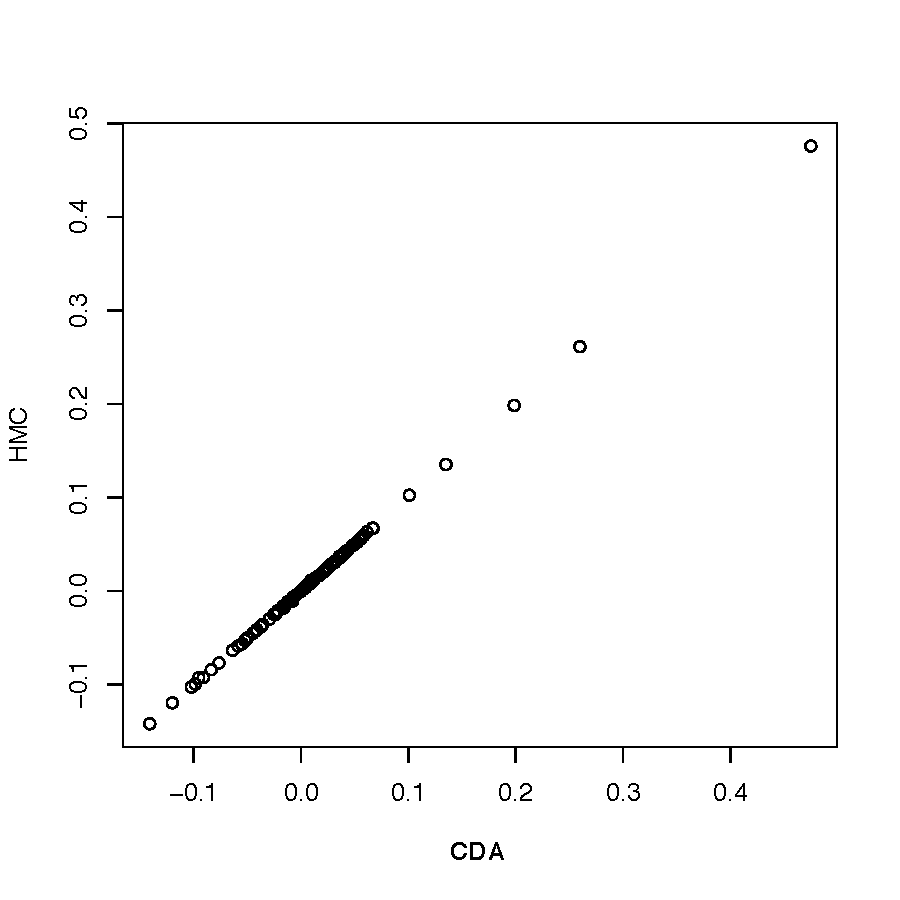
\includegraphics[width=1\textwidth]{CDAvsHMC_mean.pdf}
 \caption{Comparing posterior means for $\beta_1,\dots \beta_{95}$ from the HMC and CDA.}
 \end{subfigure}
  \hfill 
 \begin{subfigure}[b]{0.45\textwidth}
 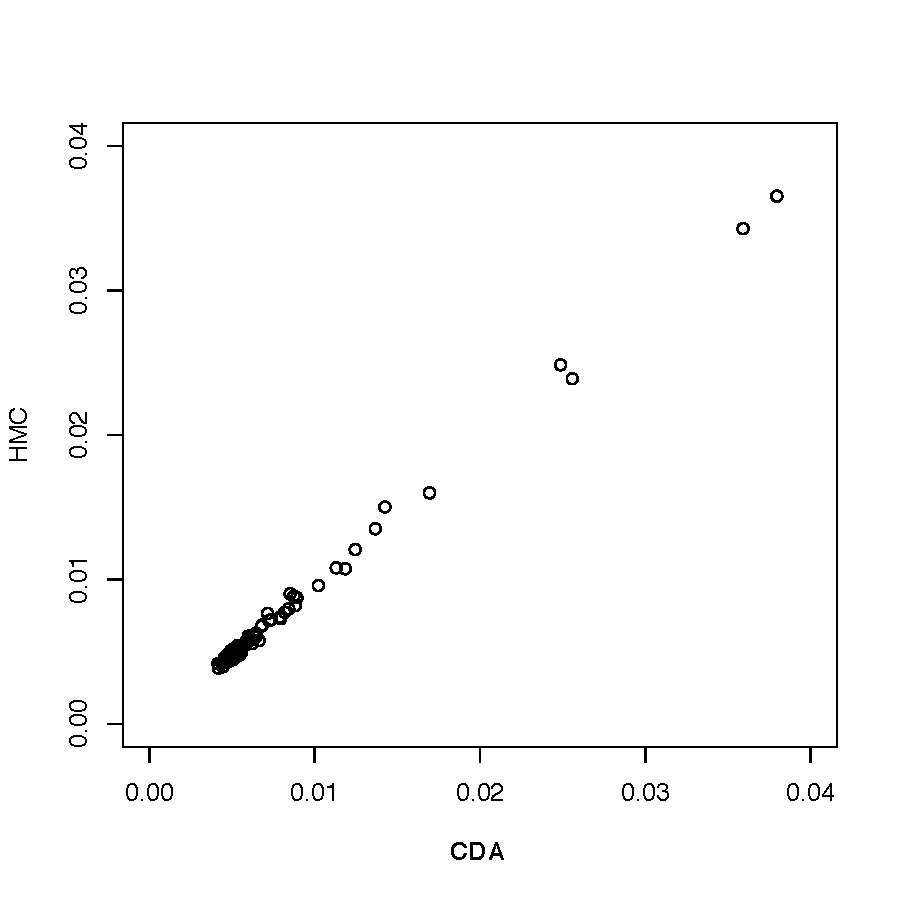
\includegraphics[width=1\textwidth]{CDAvsHMC_sd.pdf}
 \caption{Comparing posterior standard deviation for $\beta_1,\dots \beta_{95}$ from the HMC and CDA.}
 \end{subfigure}  
 \caption{The results from CDA and HMC agree very well.}
 \end{figure}

\subsection{Mixing of HMC}


 \begin{figure}[H]
 % \centering
   \begin{subfigure}[b]{0.45\textwidth}
 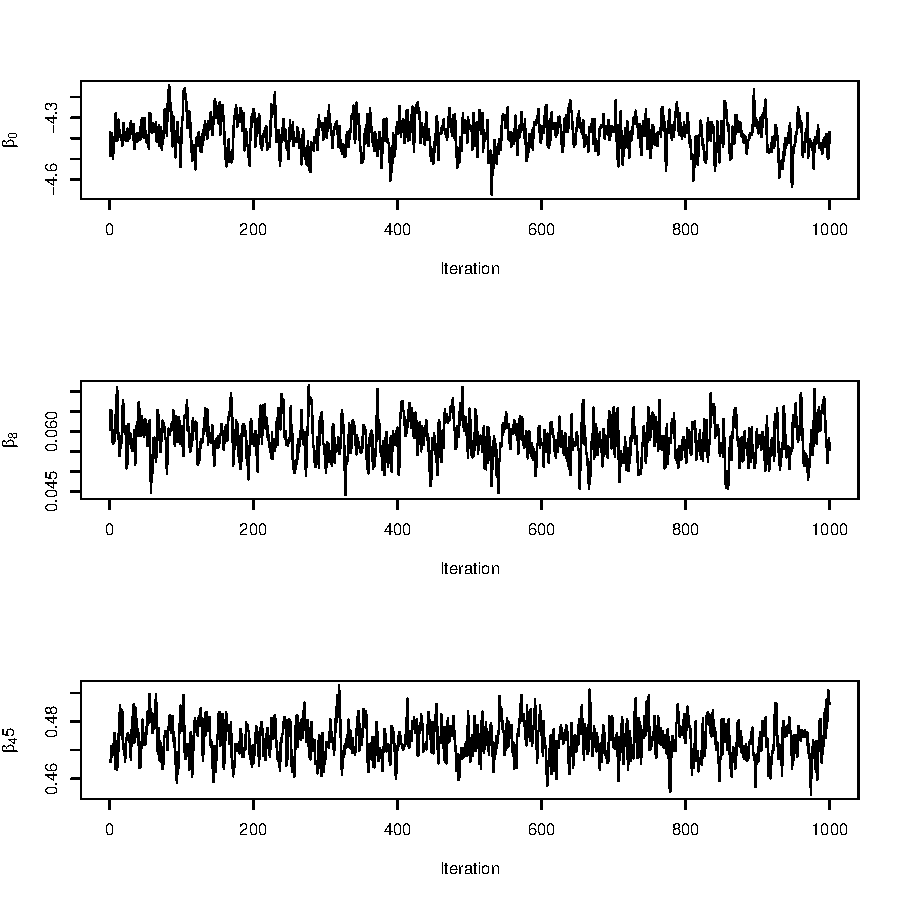
\includegraphics[width=1\textwidth]{traceplot_poisson_ada.pdf}
 \caption{Traceplots}
 \end{subfigure}
  \hfill 
 \begin{subfigure}[b]{0.45\textwidth}
 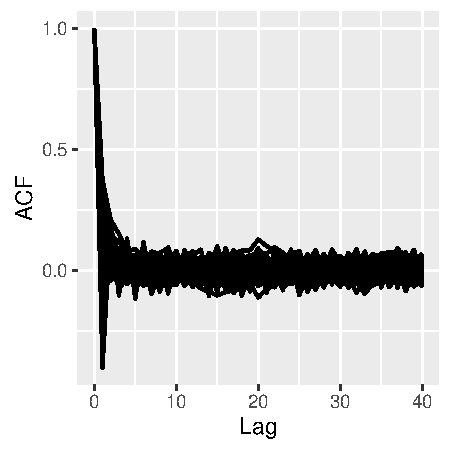
\includegraphics[width=1\textwidth]{poisson_hmc_acf.pdf}
 \caption{Autocorrelation}
 \end{subfigure}  
 \caption{The posterior estimates produced by HMC.}
 \end{figure}
 
 

\subsection{Bound on the Poisson Log Linear Model}



\begin{theorem}
The log-distance between the approximation and exact density in the Poisson log-linear model for each $y_i$ has $\log\frac{\pi_{r_i}(X_i^T\beta|y_i)}{\pi(X_i^T\beta|y_i)} \le     r_i \frac{\exp(2 X_i^T\beta)}{2}$. In order to have $\delta(P,P_r)\le\epsilon$ for each $y_i$, it suffices to have $r_i \le \frac{4\epsilon^2}{\exp(2 X_i^T\beta)}$, and additionally $r_i<\frac{1}{y_i-1}$ if $y_i>1$.
\end{theorem}

Using $\tau_i=1/r_i$ to compare with the large $\lambda$ in the original DA, when  $X_i^T\beta>0$, the lower bound provided above gives a more sensible choice about the smallest number large enough to bound the error; when $X_i^T\beta<0$, it takes a lower bound $ \frac{exp(2X_i^T\beta)}{4\epsilon^2}\ll \lambda$ and gives significant variance increase.  

\subsection{Probit Link}

It is not always viable to analytically optimize $r$ for a good balanace between approximation and mixing rate, like we did for the logistic and Poisson-log-Normal. In order to demonstrate the generality of the CDA approach, we present a numeric solution using the probit link function. The strategy is slightly different: we first make the alternative amplified chain exact with Metropolis-Hastings accept-reject sampling, then we adapt $r$ to increase the acceptance rate. Letting $r$ start from a value associated with large variance, then reducing it individually for high acceptance, is associated with reducing distance between the original and alternative. Therefore, this is phylosophically similar to the procedures we carried out above. As $r_i$ does not influence the accuracy of approximation, we can simply stop the adaptation of $r$ after tuning to ensure ergodicity.

The original DA approach for probit link $y_i\sim Bern( \Phi(X_i^T\beta))$, where $\Phi(x)=\int_{-\infty}^{x} \frac{1}{\sqrt{2{\pi}}} \exp{-\frac{t^2}{2}} dt$, is based on the following integration \citep{albert1993bayesian}:


\begin{equation}
\begin{aligned}
p(\beta,y_i) = \int_{\mathcal{Z}}  ({1}_{z_i \ge 0, y_i=1}+{1}_{z_i<0, y_i=0} )\mathcal{N}( dz_i|X_i^T\beta, 1).
\end{aligned}
\end{equation}
The sampling proceeds by alternatively updating $z_i$ from truncated normal distribution  $\mathcal{N}( z_i|X_i^T\beta, 1) ({1}_{z_i \ge 0, y_i=1}+{1}_{z_i<0, y_i=0} )$, and $\beta$ from a multivariate normal distribution $f(\beta|Z) =\mathcal{N}( \beta|(X^T X)^{-1})^{-1}(X^T Z), (X^T X )^{-1})$. The sampling can be very inefficient due to the light tails of the normal density.

To construct the CDA, we simply replace the scale of the truncated normal $z_i$ with an $r_i \ge 1$. With  $R=diag\{r^2_i\}$, this effectly increase the variance of $\beta$ to $(X^T R^{-1} X )^{-1}$. To correct the incurred error, we move the truncation point of $z_i$ from $0$ to $(1-r_i)X_i^T\beta$:

\begin{equation}
\begin{aligned}
q(\beta, y_i, r_i) = & \int_{\mathcal{Z}}  ({1}_{z_i \ge (1-r_i)X_i^T\beta, y_i=1}+{1}_{z_i<(1-r_i)X_i^T\beta, y_i=0} )\mathcal{N}( dz_i|X_i^T\beta, r_i^2).
\end{aligned}
\end{equation}

Unlike the correction term in Poisson and logistic cases that only involves $r_i$, in this case it involves $\beta$ directly so that $q(\beta, y_i, r_i)=p(\beta,y_i)$ for any $r_i \ge 1$. For the posterior sampling, the truncation is easy to accommodate when sampling $z_i$ individually; but not so much when sampling $\beta$. To solve this, we generate the proposal from the untruncated distribution and apply Metropolis-Hastings criterion. We list the algorithm as below:

\begin{algorithm}
		\caption{Probit CDA}
		\label{probit_algorithm}
		    \begin{algorithmic}

		\State \For{ $step=1\ldots N_{steps}$ }
		\State 1. Sample $z_i$ from  $ ({1}_{z_i \ge (1-r_i)X_i^T\beta, y_i=1}+{1}_{z_i<(1-r_i)X_i^T\beta, y_i=0} )\mathcal{N}( X_i^T{\beta}, r_i^2)$;\\
		\State 2. Sample $\beta'$ from  $\mathcal{N}( (X^T R^{-1} X )^{-1}(X^T R^{-1} {Z}), (X^T R^{-1} X )^{-1})$ with $R=diag\{r^2_i\}$; \\
		\State 3. Compute $\prod_i \Delta_i=\frac{p(\beta',y_i)T_i(\beta'\rightarrow \beta)}{p(\beta,y_i)T_i(\beta\rightarrow \beta')}$ where the transition kernel $T_i(\beta \rightarrow \beta')= [ \{1- \Phi(\mu_i)\} {1}_{y_i=1}+ \Phi(\mu_i) {1}_{y_i=0} ]$ with $\mu_i = \frac{\sqrt 2}{r_i}\{    (1/2-r_i)X^T_i\beta -1/2 X^T_i\beta'\}$. Update $\beta$ to $\beta'$ if a random uniform $U< \prod_i \Delta_i$;
		\EndFor
		\end{algorithmic}
\end{algorithm}

The derivation of the transition kernel is postponed to the appendix. When the proposal is accepted, the update would have lower autocorrelation for linear function $s(\beta)$ such as the individual $\beta_0$,$\beta_1$,...,or $\beta_p$, as long as at least one $r_i > 1$. Therefore, it is useful to increase $\Delta_i$ individually so that the overall acceptance rate is high. As an empirical solution, we start with a moderately large value for all $r_i$ (e.g. 100); during the tuing period, we set $r_i^{(k+1)} = 1 \vee \{ r_i^{(k)} (\Delta_i \wedge 1)\}$ so that for those with $\Delta_i < 1$ will have $r_i$ reduced. After the tuning, we fix the $r_i$ in order to have ergodicity of the chain.



\begin{algorithm}[H]
		\caption{Logistic CDA}
		\label{logistic_algorithm}
		    \begin{algorithmic}
		\State \For{ $K=1\ldots N_{steps}$ }
		\State 1. Sample $z_i$ from   $\mathcal{PG}(r_i, X_i^T\boldsymbol\beta-\log(r_i))$; \\
		\State 2. Sample $\boldsymbol\beta$ from $\mathcal{N}\big[ (X^T diag\{z_i\} X)^{-1} (X^T  \big \{ y_i - r_i/2 + z_i \log(r_i) \big\} ),(X^T diag\{z_i\} X )^{-1} \big]$;\\
		\State 3. Update $r_i= 1 \wedge \tau sup_{k\le K}\exp(X_i^T\boldsymbol\beta^{(K)})$;\\
		\EndFor
		\end{algorithmic}
\end{algorithm}


\end{document}





The second acceleration strategy is useful when the latent variable $z$ is strongly correlated to a function of the parameters (e.g. $f(\theta_1)= X^T\theta_1$ where $\theta_1=\beta$). In these scenarios, conditioning the parameter $\theta_1$ on a difference term such as $z' = z-f(\theta_1)$ or $z/f(\theta_1)$ in $\pi( \theta_1|z', y, \theta_2)$ could change the form of the distribution. The change could possibly  prevent $f(\theta_1)$ from concentrating near $z$. This is especially common when $\theta_1$ is conditionally independent with $y$ given $z$, but not so given $z'$.


\begin{algorithm}[H]
		\caption{Difference based CDA}
		\label{integration_cda}
		    \begin{algorithmic}
		\State \For{ $step=1\ldots N_{Steps}$ }
		\State Sample $z$ from $\pi(z|\theta_1,\theta_2, y)$;
		\State Sample $\theta_2$ from $\pi(\theta_2|z, y,\theta_1)$;
		\State Compute $z'$ as the difference between $z$ and $f(\theta_1)$;
		\State Sample $\theta_1$ from $\pi(\theta_1|z',\theta_2, y)$;
		\EndFor
		\end{algorithmic}
\end{algorithm}


{\bf Example 2: Generalized Linear Mixed Model}

As an illustration, consider a logistic regression with subject random effects $\pi(y_i | x_i, \beta, \sigma^2 ) = \frac{\exp(x_i^T \beta + \gamma_i )^{y_i}}{1+exp(x_i^T \beta + \gamma_i )}$, with $\gamma_i\sim N(0, \sigma^2)$ as the random effects. With latent variable $z_i = x_i^T \beta + \gamma_i$, the sampling can be proceeded

 out $\theta_1$ in the conditional distribution $\pi(z|\theta_1,\theta_2, y)$. If the posterior of $\pi(\theta_1| z, y, \theta_2)$ is in closed-form, the parameter can be marginalized out to $\pi(z,\theta_2|y) =\int\pi(z,\theta_1,\theta_2|y)d\theta_1$. As shown in Algorithm~\ref{integration_cda}, CDA samples both $z$ and $\theta_2$ from the marginal distributions, then sample $\theta_1$ from the full conditional distribution.



\begin{figure}[H]
 % \centering
 \begin{subfigure}[b]{0.49\textwidth}
 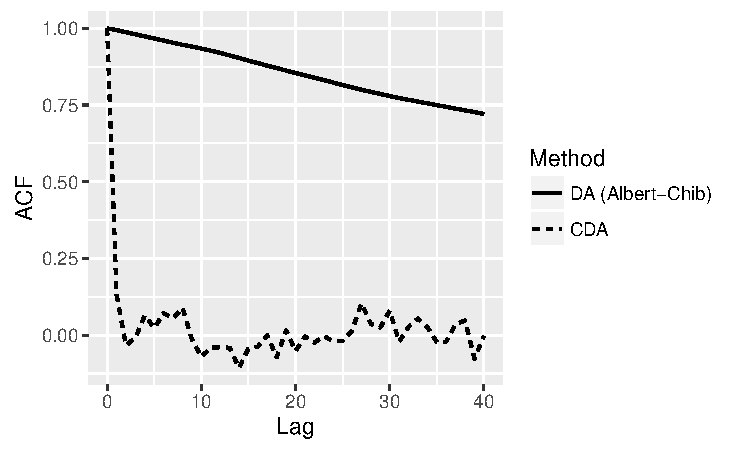
\includegraphics[width=1\textwidth]{ordered_probit_acf.pdf}
  \caption{Autocorrelation function (ACF) illustrating mixing performance of the CDA algorithm for logistic mixed effect model.}
   \label{probit_demo_rate}
\end{subfigure}
 \caption{Panel (a) demonstrates mixing and panel (b) compares marginal and conditional variances for calibrated  \cite{albert1993bayesian} in rare binary data case.}
 \end{figure}
 
 
 


proposed the $\pi(y|\theta) \propto \exp\{(y- \frac{n}{2})\theta\}\int \exp(- \frac{z \theta^2}{2})\mathcal{PG}(z|n, 0) dz$, where $\mathcal{PG}$ is the density of the Polya-Gamma distribution. The sampling is carried out by first updating the latent variable from $\pi(z|\theta)=\mathcal{PG}(n,\theta)$, then the parameter from the conditional distribution $\pi(\theta|z)=\mathcal{N}\{ z^{-1}(y-\frac{n}{2}), z^{-1}\}$. 

Similar to probit link, when $y$ is fixed and the sample size $n$ increases, the probability of positive outcomes becomes very small with the parameter variance decreases at a rate of $\mbox{var}(\theta|y)$ approximately $O(1/\log n)$, while the conditional variance $\mbox{var}(\theta|z,y)=z^{-1}$ with  $\mathbb{E}z =\frac{n}{2|\theta|}{\tanh(|\theta|/2)}$, decreases much faster in $O(1/n)$. The different rates cause slow mixing issue.

To calibrate this algorithm, $z$ is replaced with another Polya-Gamma random variable with smaller expectation $z'\sim\mathcal{PG}(n/r,0)$ with $r\ge 1$. As the integration would lead to $\pi'_r(y|\theta)\propto \frac{\exp(\theta y)}{\{1+ \exp(\theta)\}^{n/r}}$, to minimize the bias,  $\theta$ is shifted by $\log r$. This is based on the Taylor expansion $\{1+ r\exp(\theta)\}^{1/r} = \exp \{  \exp(\theta) - O(r\exp(2\theta)) \}$ for all $r>\exp(-\theta)$, so that the log density difference between any $r$ and the default $r=1$ is always in $O(r\exp(2\theta))$. This generates the CDA for the logistic regression $\pi_r(\theta|y) \propto \exp\{(y- \frac{n/r}{2})(\theta+\log r)\}\int \exp(- \frac{z' (\theta+\log r)^2}{2})\mathcal{PG}(z|n/r, 0) dz'$.

The CDA updates $z'$ from $\mathcal{PG}(n/r, \theta+\log r)$ and $\theta$ from $\mathcal{N}\{ z'^{-1}(y-\frac{n}{2})-\log r, z'^{-1}\}$ in each MCMC iteration. The marginal density is $\pi_r(\theta|y)=\frac{\Gamma(n/r+1)}{\Gamma(n/r-y+1)\Gamma(y+1)}\frac{\exp ( \theta+\log r)^y}{\{1+ \exp ( \theta+\log r)\}^{n/r}}$, with $y< n/r+1$. As one intuitive interpretation, the new density is close to  the $y$ successes of $n/r$ draws that approximates the original binomial density of $y$ successes of $n$ draws. The parameter $r$ reduces the large difference between the number of successes and the total draw hence avoids the slow mixing problem.

\begin{theorem}
The log-distance between the approximation and exact density in the binomial logistic link has $\log\frac{\pi_{r_i}(\theta|y)}{\pi(\theta|y)} \le     (r-1) \frac{n \exp(2\theta)}{2}   1_{\exp(\theta)< 1/r}$. In order to have $\delta(P,P_r)\le\epsilon$, it suffices to have $r\le \frac{4\epsilon^2}{n\exp(2\theta)}$ if $\theta<0$, $r=1$ otherwise.
\end{theorem}

It should be stressed that the upper bound on $r$ is quite large for calibrating slow mixing. With an empirical estimate $\exp(\theta)\approx y/n$, the upper bound for $r$ is approximately $4n\epsilon^2/y^2$. 

On the ergodicity, let $\{r_k\}_{k=1\ldots K}$ be the adaptive sequence of working parameters in the first $K$ steps. As each $r_k$ is associated with a binomial density with Polya-Gamma augmentation, they are all uniformly ergodic \citep{choi2013polya}. For the diminishing adaptation condition, it can be first observed that the approximation error is monotonically increasing in $r>1$. This suggests a non-increasing sequence of $r_k$ will always guarantees the previous posterior samples is in the neighborhood of the true density. Let $\varTheta^*_K=\{\theta^{(1)},\ldots,\theta^{(K)}\}$ be the posterior collected in the first $K$ iterations, let $r_k= \underset{\theta\in \varTheta_K^*}{\min}\frac{4\epsilon^2}{n\exp(2\theta)} = \frac{4\epsilon^2}{n\exp(2\underset{\theta\in \varTheta_K^*}{\max}\theta)}$. As $\underset{\theta\in \varTheta_K^*}{\max}\theta$ converges in probability as $K\rightarrow \infty$, $r_k$ converges as well. These two conditions ensure that the CDA for logistic link is uniformly ergodic.


\section{Illustrations}
%
%
%\subsection{Exact Tempering: Binomial Regression with Probit Link}
%We first consider a toy example in which an exact CDA algorithm can be implemented without approximation error, so that the impact of $r$ on improving computational efficiency can be isolated.  Consider a binomial likelihood with probit link: $\prod_{i=1}^{n}\pi(y_i|\theta)= \prod_{i=1}^n \Phi(\theta)^{y_i} \{ 1-\Phi(\theta) \} ^{(1-y_i)}$, where $\Phi(\theta)$ is the standard normal cumulative distribution function and $\pi(\theta) \propto 1$. The \cite{albert1993bayesian} sampler alternately draws each latent variable $z_i$ independently from the truncated normal distributions, $\pi(z_i|\theta,y_i=0)= \mathcal{N}_{(-\infty,0)}( z_i| \theta, 1)$ and $\pi(z_i | \theta, y_i=1) = \mathcal{N}_{(0,\infty)}( z_i| \theta, 1)$, and then the parameter $\theta$ from $\pi(\theta|z,y)=\mathcal{N}( \theta | \overline{z}, 1/n )$.  Slow mixing is particularly problematic 
%when $\sum_{i=1}^n y_i$ is small even when $n$ is very large, which is common in rare event applications.
%
%The CDA algorithm replaces the conditional variance $1/n$ with $r/n$, leading to $\pi'_r( \theta |y ) = \prod_{i=1}^n \Phi(\theta/\sqrt{r})^{y_i} \{ 1-\Phi(\theta/\sqrt{r}) \} ^{(1-y_i)}$.  As a second step to remove the bias, we replace $y_i = 1(z_i > 0)$ with $y_i = 1\{ z_i > (1-\sqrt{r})\theta \}$.  The resulting CDA sampler first draws latent variables 
%independently from $z_i \sim \mathcal{N}_{\big(-\infty, (1-\sqrt{r})\theta \big)}( \theta, r )$ for $y_i=0$ and 
%$z_i \sim \mathcal{N}_{\big( (1-\sqrt{r})\theta, \infty \big)}( \theta, r )$ for $y_i=1$, 
%and then $\theta \sim \mathcal{N}_{\big( \underset{{i:y_i=1}}{\max}z_i /(1-\sqrt{r}) ,  \underset{i:y_i=0}{\min}z_i /(1-\sqrt{r}) \big) }( \overline{z}, r/n )$.
%There is no approximation error as $\pi(\theta|y)=\pi_r(\theta|y)$ holds for all $r$, with the original  \cite{albert1993bayesian} approach obtained for $r=1$.  As $r$ increases, the conditional variance of the latent data $z_i$ increases while the size of the support of the conditional of $\theta$ shrinks.  
%
%For illustration, we let $\sum_i y_i=1$ (to mimic rare event data), $n=10,000$ and applied CDA with different values of $r$. As shown in Figure~\ref{probit_demo_acf}, the original \cite{albert1993bayesian} algorithm ($r=1$) suffers from extremely slow mixing, attributable to the large gap between the conditional and marginal variance of $\theta$ shown in  Figure~\ref{probit_demo_rate}.  By increasing $r$, mixing performance is substantially improved, with the optimal value reached near $r = 1,000 \approx n/\log(n)$, which corresponds to the ratio of marginal and conditional asymptotic variances of $\theta$.
%
%\begin{figure}[H]
% % \centering
% \begin{subfigure}[b]{0.49\textwidth}
% 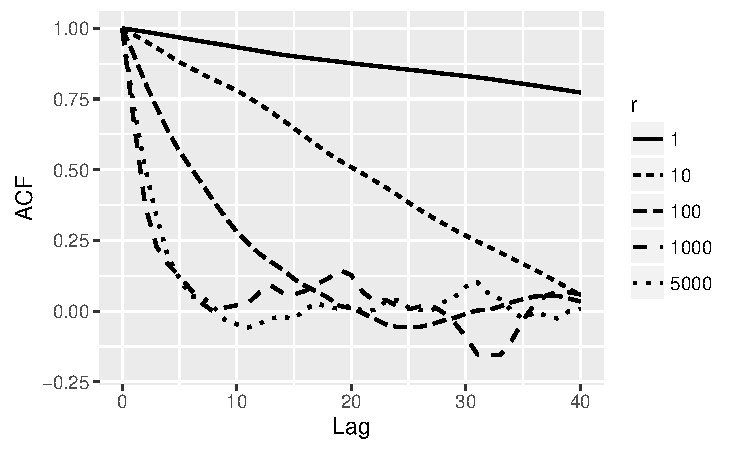
\includegraphics[width=0.8\textwidth]{probit_demo_acf.pdf}
%  \caption{Autocorrelation function (ACF) illustrating mixing performance of the CDA algorithm for rare binary events data.}
%   \label{probit_demo_acf}
%\end{subfigure}
% \hfill
% \begin{subfigure}[b]{0.49\textwidth}
% 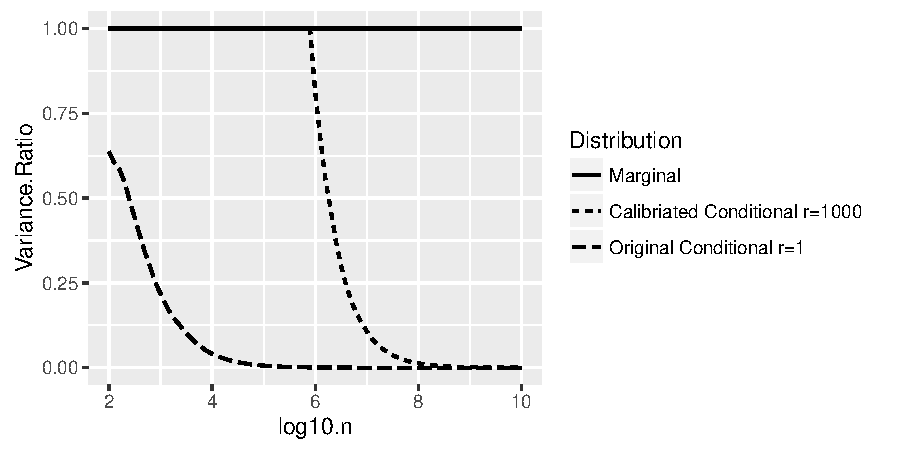
\includegraphics[width=1\textwidth]{probit_rate.pdf}
%  \caption{Comparing the ratios $\mbox{var}_r( \theta | z,y)/\mbox{var}( \theta | y)$ for different $r$ as a function of $\log_{10} n$.}
%   \label{probit_demo_rate}
%\end{subfigure}
% \caption{Panel (a) demonstrates mixing and panel (b) compares marginal and conditional variances for calibrated  \cite{albert1993bayesian} in rare binary data case.}
% \end{figure}
% 






